\documentclass[UTF8,a4paper,11pt]{ctexart}
\usepackage[margin=2.2cm,headheight=15pt]{geometry}
\usepackage{amsmath,amssymb,amsthm,bm,mathtools}
\usepackage{booktabs,tabularx,array,multirow,makecell}
\usepackage{graphicx,xcolor}
\usepackage{tikz}
\usetikzlibrary{arrows.meta,positioning,calc}
\usepackage[section]{placeins}
\usepackage{algorithm,algpseudocode}
\usepackage{float,caption,subcaption,fancyhdr,microtype,enumitem}
\usepackage[colorlinks=true,linkcolor=teal,citecolor=teal,urlcolor=teal]{hyperref}

\setlength{\parindent}{2em}
\setlength{\parskip}{0.25em}
\setlength{\emergencystretch}{2em}
\linespread{1.2}
\renewcommand{\arraystretch}{1.15}
\captionsetup{font=small,labelsep=quad}
\setlist{itemsep=0.15em,topsep=0.3em}

% pseudo-code keeps the English keywords (for, if, return, ...)
\floatname{algorithm}{算法}
\algrenewcommand\algorithmicrequire{\textbf{Input:}}
\algrenewcommand\algorithmicensure{\textbf{Output:}}
\algrenewcommand{\algorithmiccomment}[1]{\hfill$\triangleright$ #1}

\newcommand{\E}{\mathbb E}
\newcommand{\ind}{\mathbf 1}
\newcommand{\seq}{\mathrm{seq}}
\newcommand{\Pol}[1]{\textsf{#1}}
\newcommand{\AlgOne}{\Pol{Alg1}}
\newcommand{\Greedy}{\Pol{Greedy}}
\newcommand{\LPFD}{\Pol{LP-FD}}
\newcommand{\LPDual}{\Pol{LP-Dual}}
\newcommand{\LPCount}{\Pol{LP-Count}}
\newcommand{\IIDDP}{\Pol{IID-DP}}
\newcommand{\SeqDP}{\Pol{Seq-DP}}

\theoremstyle{definition}   % upright body text suits Chinese
\newtheorem{proposition}{命题}
\newtheorem{definition}{定义}
\newtheorem{example}{算例}
\renewcommand{\proofname}{证明}

\pagestyle{fancy}
\fancyhf{}
\fancyhead[L]{\small 库存约束下的在线 Top-$K$ 推荐}
\fancyhead[R]{\small 线性规划机会成本与滚动前瞻}
\fancyfoot[C]{\thepage}

% generated by code/make_assets.py -- do not edit by hand
\newcommand{\AlgOneER}{693.394}
\newcommand{\AlgOneLossGreedy}{2.156}
\newcommand{\AlgOneOOS}{6.29}
\newcommand{\AlgOneSdIid}{8.364}
\newcommand{\AlgOneSdPerm}{0.000}
\newcommand{\BlockCount}{696.999}
\newcommand{\BlockDual}{683.029}
\newcommand{\BlockEconeCount}{0.857}
\newcommand{\BlockEconeDual}{2.360}
\newcommand{\BlockEconeFD}{3.220}
\newcommand{\BlockEconeGreedy}{0.857}
\newcommand{\BlockEconeIID}{3.714}
\newcommand{\BlockEconeSeq}{0.858}
\newcommand{\BlockFD}{674.747}
\newcommand{\BlockGreedy}{696.997}
\newcommand{\BlockIID}{670.601}
\newcommand{\BlockOTTCount}{690.984}
\newcommand{\BlockOTTDual}{694.199}
\newcommand{\BlockOTTEconeCount}{1.424}
\newcommand{\BlockOTTEconeSeq}{0.901}
\newcommand{\BlockOTTFD}{694.200}
\newcommand{\BlockOTTGreedy}{694.050}
\newcommand{\BlockOTTIID}{693.735}
\newcommand{\BlockOTTSeq}{694.543}
\newcommand{\BlockOTWCount}{690.307}
\newcommand{\BlockOTWDual}{693.588}
\newcommand{\BlockOTWEconeCount}{1.483}
\newcommand{\BlockOTWEconeSeq}{0.948}
\newcommand{\BlockOTWFD}{693.626}
\newcommand{\BlockOTWGreedy}{693.395}
\newcommand{\BlockOTWIID}{693.126}
\newcommand{\BlockOTWSeq}{693.946}
\newcommand{\BlockSeq}{697.000}
\newcommand{\ContribOneDual}{9.029}
\newcommand{\ContribOneShare}{89}
\newcommand{\ContribThreeDual}{-0.346}
\newcommand{\ContribTwoDual}{1.423}
\newcommand{\CorrDualLastTwenty}{0.73}
\newcommand{\CorrFDLastTen}{-0.46}
\newcommand{\CorrGreedyLastTwenty}{0.76}
\newcommand{\DemandOneLeft}{0.923}
\newcommand{\DemandOneSd}{4.38}
\newcommand{\DemandOneShort}{28.4}
\newcommand{\DualBeatsFDIid}{60.8}
\newcommand{\DualBeatsFDPerm}{65.4}
\newcommand{\DualBeatsGreedyIid}{99.8}
\newcommand{\DualBeatsGreedyPerm}{99.8}
\newcommand{\DualBeatsIIDIid}{15.2}
\newcommand{\DualBeatsIIDPerm}{13.8}
\newcommand{\DualFDAvg}{0.403}
\newcommand{\DualFDWins}{4}
\newcommand{\DualGreedyAvg}{0.344}
\newcommand{\DualGreedyMax}{0.428}
\newcommand{\DualGreedyMin}{0.291}
\newcommand{\DualMinusGreedyIid}{0.393}
\newcommand{\DualMinusGreedyPerm}{0.324}
\newcommand{\ERAlg}{693.394}
\newcommand{\ERCount}{695.768}
\newcommand{\ERDual}{695.894}
\newcommand{\ERFD}{695.490}
\newcommand{\ERGreedy}{695.550}
\newcommand{\ERIID}{695.862}
\newcommand{\ERSeq}{696.062}
\newcommand{\EconeAlg}{0.923}
\newcommand{\EconeCount}{0.943}
\newcommand{\EconeDual}{0.903}
\newcommand{\EconeFD}{0.987}
\newcommand{\EconeGreedy}{0.911}
\newcommand{\EconeIID}{0.935}
\newcommand{\EconeSeq}{0.904}
\newcommand{\EcthreeAlg}{13.00}
\newcommand{\EcthreeCount}{12.56}
\newcommand{\EcthreeDual}{12.61}
\newcommand{\EcthreeFD}{12.51}
\newcommand{\EcthreeGreedy}{12.66}
\newcommand{\EcthreeIID}{12.55}
\newcommand{\EcthreeSeq}{12.57}
\newcommand{\EctwoAlg}{6.17}
\newcommand{\EctwoCount}{6.18}
\newcommand{\EctwoDual}{6.18}
\newcommand{\EctwoFD}{6.19}
\newcommand{\EctwoGreedy}{6.17}
\newcommand{\EctwoIID}{6.18}
\newcommand{\EctwoSeq}{6.19}
\newcommand{\ExactSeconds}{0.16}
\newcommand{\FirstPeriodF}{702.54}
\newcommand{\FluidGap}{9.938}
\newcommand{\FluidGapIid}{9.262}
\newcommand{\FluidGapMax}{10.525}
\newcommand{\FluidGapMin}{9.513}
\newcommand{\FluidGapPerm}{9.705}
\newcommand{\FluidShare}{98.3}
\newcommand{\FmaxIid}{729.2}
\newcommand{\FmaxPerm}{706.0}
\newcommand{\FmeanIid}{703.396}
\newcommand{\FmeanPerm}{706.000}
\newcommand{\FminIid}{660.0}
\newcommand{\FminPerm}{706.0}
\newcommand{\GavgAlg}{12.606}
\newcommand{\GavgAlgIid}{12.522}
\newcommand{\GavgAlgPerm}{12.606}
\newcommand{\GavgCount}{10.232}
\newcommand{\GavgDual}{10.106}
\newcommand{\GavgDualIid}{9.513}
\newcommand{\GavgDualPerm}{9.902}
\newcommand{\GavgFD}{10.510}
\newcommand{\GavgFDIid}{9.711}
\newcommand{\GavgFDPerm}{10.200}
\newcommand{\GavgGreedy}{10.450}
\newcommand{\GavgGreedyIid}{9.906}
\newcommand{\GavgGreedyPerm}{10.226}
\newcommand{\GavgIID}{10.138}
\newcommand{\GavgIIDIid}{9.370}
\newcommand{\GavgIIDPerm}{9.801}
\newcommand{\GavgSeq}{9.938}
\newcommand{\GmaxAlg}{12.606}
\newcommand{\GmaxCount}{11.147}
\newcommand{\GmaxDual}{10.740}
\newcommand{\GmaxFD}{11.058}
\newcommand{\GmaxGreedy}{11.168}
\newcommand{\GmaxIID}{10.815}
\newcommand{\GmaxSeq}{10.525}
\newcommand{\HoldBlockDual}{13.226}
\newcommand{\HoldBlockFD}{20.925}
\newcommand{\HoldBlockGreedy}{0.000}
\newcommand{\HoldBlockIID}{25.428}
\newcommand{\HoldThetaSevenDual}{0.001}
\newcommand{\HoldThetaSevenFD}{0.041}
\newcommand{\HoldThetaSevenGreedy}{0.000}
\newcommand{\HoldThetaSevenIID}{0.135}
\newcommand{\IIDSeconds}{0.5}
\newcommand{\KERoneAlg}{462.772}
\newcommand{\KERoneDual}{484.848}
\newcommand{\KERoneFD}{487.070}
\newcommand{\KERoneGreedy}{478.001}
\newcommand{\KERoneIID}{491.992}
\newcommand{\KERthreeAlg}{727.810}
\newcommand{\KERthreeDual}{727.810}
\newcommand{\KERthreeFD}{727.810}
\newcommand{\KERthreeGreedy}{727.810}
\newcommand{\KERthreeIID}{727.810}
\newcommand{\KERtwoAlg}{693.394}
\newcommand{\KERtwoDual}{695.894}
\newcommand{\KERtwoFD}{695.490}
\newcommand{\KERtwoGreedy}{695.550}
\newcommand{\KERtwoIID}{695.862}
\newcommand{\KFone}{492}
\newcommand{\KFthree}{734}
\newcommand{\KFtwo}{706}
\newcommand{\KVone}{491.992}
\newcommand{\KVthree}{727.810}
\newcommand{\KVtwo}{696.062}
\newcommand{\LargeAlgOneMax}{94.6}
\newcommand{\LargeAlgOneMin}{81.9}
\newcommand{\LargeGreedyMin}{91.1}
\newcommand{\LargeInstances}{80}
\newcommand{\LargePairMax}{0.32}
\newcommand{\LargePairMin}{-0.07}
\newcommand{\LargeRows}{50}
\newcommand{\LargeSigLosses}{3}
\newcommand{\LargeSigWins}{6}
\newcommand{\LargeTimeFD}{25.6}
\newcommand{\LargeTimeMedian}{3.27}
\newcommand{\LargeTimeP}{5.06}
\newcommand{\LargeVars}{600}
\newcommand{\LavgAlg}{2.669}
\newcommand{\LavgAlgIid}{3.260}
\newcommand{\LavgAlgPerm}{2.901}
\newcommand{\LavgCount}{0.295}
\newcommand{\LavgDual}{0.169}
\newcommand{\LavgDualIid}{0.251}
\newcommand{\LavgDualPerm}{0.197}
\newcommand{\LavgFD}{0.572}
\newcommand{\LavgFDIid}{0.449}
\newcommand{\LavgFDPerm}{0.495}
\newcommand{\LavgGreedy}{0.513}
\newcommand{\LavgGreedyIid}{0.644}
\newcommand{\LavgGreedyPerm}{0.520}
\newcommand{\LavgIID}{0.201}
\newcommand{\LavgIIDIid}{0.108}
\newcommand{\LavgIIDPerm}{0.096}
\newcommand{\LavgSeq}{0.000}
\newcommand{\LmaxDualIid}{1.370}
\newcommand{\LmaxDualPerm}{0.561}
\newcommand{\LmaxFDIid}{3.180}
\newcommand{\LmaxFDPerm}{3.485}
\newcommand{\LossBlockDual}{13.971}
\newcommand{\LossBlockFD}{22.253}
\newcommand{\LossBlockGreedy}{0.003}
\newcommand{\LossBlockIID}{26.400}
\newcommand{\LossEndDual}{0.067}
\newcommand{\LossEndFD}{0.476}
\newcommand{\LossEndGreedy}{0.068}
\newcommand{\LossEndIID}{0.155}
\newcommand{\LossHoldDual}{0.010}
\newcommand{\LossHoldFD}{0.530}
\newcommand{\LossHoldGreedy}{0.000}
\newcommand{\LossHoldIID}{0.155}
\newcommand{\LossIdentityErr}{8\times10^{-13}}
\newcommand{\LossKoneDual}{7.145}
\newcommand{\LossKoneFD}{4.923}
\newcommand{\LossKoneGreedy}{13.991}
\newcommand{\LossKoneIID}{0.000}
\newcommand{\LossMidDual}{0.099}
\newcommand{\LossMidFD}{0.093}
\newcommand{\LossMidGreedy}{0.438}
\newcommand{\LossMidIID}{0.045}
\newcommand{\LossSellDual}{0.112}
\newcommand{\LossSellFD}{0.010}
\newcommand{\LossSellGreedy}{0.357}
\newcommand{\LossSellIID}{0.020}
\newcommand{\LossThetaSevenDual}{3.609}
\newcommand{\LossThetaSevenFD}{3.888}
\newcommand{\LossThetaSevenGreedy}{8.638}
\newcommand{\LossThetaSevenIID}{0.335}
\newcommand{\MChw}{1.24}
\newcommand{\MCinside}{25}
\newcommand{\MCmaxZ}{1.59}
\newcommand{\MCpairEqual}{88.0}
\newcommand{\MCpairEqualFD}{80.1}
\newcommand{\MCpairhw}{0.12}
\newcommand{\MCtotal}{25}
\newcommand{\NewsCostMean}{10.61}
\newcommand{\NewsCostOpt}{4.62}
\newcommand{\NewsLeft}{1.06}
\newcommand{\NewsQuantile}{9}
\newcommand{\PnegDual}{35.9}
\newcommand{\PnegDualMax}{36.6}
\newcommand{\PnegDualMin}{35.1}
\newcommand{\ProbAboveFDOne}{35.8}
\newcommand{\QoneGreedyGap}{1.5}
\newcommand{\QoneLPMaxGap}{0.17}
\newcommand{\QoneLossOptHundred}{87.0}
\newcommand{\QoneLossOptTwenty}{57.1}
\newcommand{\QoneWasteTwenty}{34.7}
\newcommand{\RatioDual}{98.57}
\newcommand{\RunsHi}{72}
\newcommand{\RunsLo}{55}
\newcommand{\RunsMax}{71}
\newcommand{\RunsMin}{60}
\newcommand{\ScaleDualHwMax}{7.5}
\newcommand{\ScaleGDualMax}{10.9}
\newcommand{\ScaleGDualMin}{3.5}
\newcommand{\ScaleGapSmall}{0.36}
\newcommand{\ScaleGreedyFluid}{9.1}
\newcommand{\ScaleGreedyGapMax}{6.55}
\newcommand{\ScaleGreedyGapMaxHw}{0.55}
\newcommand{\ScaleRatioMax}{99.97}
\newcommand{\ScaleTmax}{1600}
\newcommand{\SdDual}{27.9}
\newcommand{\SellThetaSevenDual}{3.574}
\newcommand{\SellThetaSevenFD}{3.813}
\newcommand{\SellThetaSevenGreedy}{7.087}
\newcommand{\SellThetaSevenIID}{0.114}
\newcommand{\SoldOutEightyDual}{0.5}
\newcommand{\SoldOutEightyFD}{0.2}
\newcommand{\SoldOutEightyGreedy}{6.1}
\newcommand{\SoldOutEightyIID}{0.0}
\newcommand{\SoldOutEightySeq}{0.0}
\newcommand{\SoldOutEndDual}{71.6}
\newcommand{\SoldOutEndFD}{63.0}
\newcommand{\SoldOutEndGreedy}{71.7}
\newcommand{\SoldOutEndIID}{68.1}
\newcommand{\SoldOutEndSeq}{70.9}
\newcommand{\SolvesDual}{94{,}525}
\newcommand{\SolvesFD}{139{,}224}
\newcommand{\TableSeconds}{108}
\newcommand{\ThetaA}{1.05}
\newcommand{\ThetaB}{0.829}
\newcommand{\ThetaC}{0.680}
\newcommand{\ThetaEightLAlg}{12.434}
\newcommand{\ThetaEightLDual}{1.665}
\newcommand{\ThetaEightLFD}{1.643}
\newcommand{\ThetaEightLGreedy}{4.723}
\newcommand{\ThetaEightLIID}{0.328}
\newcommand{\ThetaEightW}{26.80}
\newcommand{\ThetaHalfLAlg}{7.945}
\newcommand{\ThetaHalfLDual}{1.583}
\newcommand{\ThetaHalfLFD}{1.583}
\newcommand{\ThetaHalfLGreedy}{1.796}
\newcommand{\ThetaHalfLIID}{0.003}
\newcommand{\ThetaHalfW}{80.29}
\newcommand{\ThetaOneLAlg}{2.669}
\newcommand{\ThetaOneLDual}{0.169}
\newcommand{\ThetaOneLFD}{0.572}
\newcommand{\ThetaOneLGreedy}{0.513}
\newcommand{\ThetaOneLIID}{0.201}
\newcommand{\ThetaOneW}{6.29}
\newcommand{\ThetaSevenLAlg}{18.769}
\newcommand{\ThetaSevenLDual}{3.609}
\newcommand{\ThetaSevenLFD}{3.888}
\newcommand{\ThetaSevenLGreedy}{8.638}
\newcommand{\ThetaSevenLIID}{0.335}
\newcommand{\ThetaSevenW}{41.79}
\newcommand{\ThetaSixLAlg}{15.256}
\newcommand{\ThetaSixLDual}{3.174}
\newcommand{\ThetaSixLFD}{3.174}
\newcommand{\ThetaSixLGreedy}{5.685}
\newcommand{\ThetaSixLIID}{0.067}
\newcommand{\ThetaSixW}{62.04}
\newcommand{\ThetaTwelveLAlg}{0.107}
\newcommand{\ThetaTwelveLDual}{0.006}
\newcommand{\ThetaTwelveLFD}{0.064}
\newcommand{\ThetaTwelveLGreedy}{0.012}
\newcommand{\ThetaTwelveLIID}{0.016}
\newcommand{\ThetaTwelveW}{0.35}
\newcommand{\ThetaWorstDual}{0.7}
\newcommand{\ThetaWorstDualL}{3.609}
\newcommand{\ThrDualHundred}{11}
\newcommand{\ThrFDHundred}{12}
\newcommand{\ThrIIDHundred}{23}
\newcommand{\TimeDualMedian}{0.057}
\newcommand{\TimeDualP}{0.68}
\newcommand{\TimeFDMedian}{0.055}
\newcommand{\TimeFDP}{0.90}
\newcommand{\TopFDLastTenMax}{2}
\newcommand{\TypeTwoSellKoneDual}{7.145}
\newcommand{\TypeTwoSellKoneFD}{4.923}
\newcommand{\TypeTwoSellKoneGreedy}{13.991}
\newcommand{\TypeTwoSellKoneIID}{0.000}
\newcommand{\VerifyDecisions}{300{,}000}
\newcommand{\VerifyMismatch}{0}


\title{\bfseries 库存约束下的在线 Top-$K$ 推荐\\[0.4em]
\large 基于线性规划库存机会成本的滚动前瞻策略}
\author{组员：\underline{\hspace{9cm}}}
\date{2026年11月}

\begin{document}
\maketitle
\begin{abstract}
有限库存使平台面临两个决策：售罄后用什么商品补足推荐位，以及是否把尚有库存的商品留给后续顾客。本文构造单类型算例，说明固定 Top-$K$ 推荐在 20 期内相对简单可行策略损失 47.08\% 的期望收入。对于课程实例，含库存约束的流体线性规划给出收入上界 706，商品 1 的影子价格为 9。本文据此设计滚动策略 \LPDual{}，每期按购买概率与扣除库存机会成本后的价格为有货商品排序。五份给定到达序列上，该策略的平均期望收入为 \ERDual，平均和最大期望遗憾分别为 \GavgDual{} 和 \GmaxDual，缺货推荐次数均为零。相对库存感知贪心，每条序列平均增收 \DualGreedyAvg{}（\DualGreedyRelativePct\%），与预知到达顺序的最优策略之间的平均差距由 \LavgGreedy{} 降至 \LavgDual{}，缩小 \DualSeqGapReductionPct\%。库存缩放实验表明，缺货展示在库存极少时最频繁，而把稀缺商品分配给不同顾客带来的收入差异在库存中度紧张时最大。
\end{abstract}
\noindent\textbf{关键词：}在线推荐；库存约束；流体线性规划；影子价格；动态规划

\section{引言}\label{sec:intro}
盒马等生鲜电商每天以有限的库存开始营业，营业期间无法补货。顾客打开 App 时，平台需要在几毫秒内决定推荐哪些商品。这一决定会影响后续的销售：一件稀缺商品卖给当前顾客，后面更需要它的顾客可能就买不到了。题目\cite{assignment}给出的算法 1 按单次期望收益 $r_jp_{ij}$ 为每类顾客固定推荐前 $K$ 件商品，没有考虑库存。本文围绕题目的三个问题展开：
\begin{enumerate}[label=(\arabic*)]
\item 有限库存下能否继续使用算法 1？是否存在使其收入损失超过 30\% 的例子？
\item 考虑库存约束时，离线（hindsight）模型是什么？
\item 如何设计满足库存约束、可实时运行的在线推荐算法？
\end{enumerate}

本文的主要工作与结论如下。
\begin{itemize}
\item \textbf{问题一。} 算法 1 会推荐缺货商品，违反库存可行性。本文构造了一族单类型算例，算法 1 相对可行策略的收入损失在销售期 $T\ge14$ 时超过 30\%，$T=20$ 时为 47.08\%，并随 $T$ 增大趋于 100\%。
\item \textbf{问题二。} 建立含库存约束的流体线性规划，证明其最优值是任意在线策略期望收入的上界。课程实例的最优值为 706，商品 1 的影子价格为 9。本文比较了三种离线表达，并给出了库存缩放下影子价格的变化。
\item \textbf{问题三。} 提出 \LPDual{} 策略：每期以当前库存与剩余期数重新求解一次流体线性规划，用库存约束的对偶价格作为机会成本，推荐调整后收益最高的至多 $K$ 件有货商品。策略每期只求解一个 $mn$ 维的连续线性规划，满足零缺货推荐，可以在任意 $m,n,T,K$ 下运行。
\item \textbf{评价。} 本文用库存格点上的前向递推精确计算各策略的期望收入，不含蒙特卡洛误差。五份数据上，\LPDual{} 的平均遗憾为 \GavgDual，最大遗憾为 \GmaxDual，均低于库存感知贪心策略与有限差分版本；遗憾中有 \FluidShare\% 是流体模型与随机系统之间的松弛间隙，与预知全部顾客类型的最优策略相比，策略损失只有 \LavgDual。
\item \textbf{分析。} 通过损失分解、1000 条生成序列、分块到达顺序、库存与推荐位数的灵敏度，以及销售期放大与较大实例，本文说明了各策略在何时、因何损失收入，以及流体近似的适用范围。
\end{itemize}

全文结构如下：第\ref{sec:setting}节描述问题与模型；第\ref{sec:q1}、\ref{sec:q2}、\ref{sec:policy}节依次回答三个问题；第\ref{sec:eval}节给出评价方法；第\ref{sec:exp}节报告数值实验；第\ref{sec:conclusion}节总结。附录说明程序结构与自动化测试。

\section{问题描述与模型}\label{sec:setting}

\subsection{业务场景与决策流程}
考虑一家生鲜平台在一小时营业窗口内的推荐决策。窗口被划分为 $T$ 个时段（题目实例中 $T=100$），每个时段恰有一位顾客进入 App。平台销售 $n$ 种商品，商品 $j$ 的单价为 $r_j$，营业开始时的库存为 $C_j$，窗口内无法补货。平台依据历史浏览与购买数据把顾客划分为 $m$ 种类型，任一时段到达的顾客属于类型 $i$ 的概率为 $\lambda_i$，$\sum_{i}\lambda_i=1$，因而一个窗口内类型 $i$ 的期望人数为 $T\lambda_i$。

图\ref{fig:flow}给出单个时段内的决策流程。第 $t$ 期顾客到达后，平台依次完成四个动作：
\begin{enumerate}[label=(\arabic*)]
\item 识别顾客类型 $i_t$，读取当前库存向量 $c_t=(c_{t1},\ldots,c_{tn})$ 与含本期在内的剩余期数 $T-t+1$；
\item 从有货商品中选出至多 $K$ 件组成推荐集合 $S_t$，展示给顾客；
\item 顾客浏览推荐列表，至多购买一件商品；
\item 若顾客购买商品 $j$，平台获得收入 $r_j$，库存更新为 $c_{t+1}=c_t-e_j$（$e_j$ 为第 $j$ 个单位向量）；若顾客未购买，库存保持不变。
\end{enumerate}
窗口结束时剩余商品不产生残值，平台的目标是最大化 $T$ 期的期望总收入 $R_T=\sum_{t=1}^{T}r_{J'_t}$，其中 $J'_t$ 表示第 $t$ 期实际成交的商品（未成交时该项为零）。

\begin{figure}[htbp]
\centering
\begin{tikzpicture}[
  node distance=5mm and 6mm,
  box/.style={draw=black!55, rounded corners=2pt, fill=black!3, align=center,
              minimum height=17mm, text width=32mm, font=\small},
  arr/.style={-{Stealth[length=2.2mm]}, semithick, black!70}]
\node[box] (a) {顾客到达\\识别类型 $i_t$};
\node[box, right=of a] (b) {读取在线状态\\$(i_t,\ c_t,\ T-t+1)$};
\node[box, right=of b] (c) {生成推荐集合 $S_t$\\$S_t\subseteq A(c_t)$\\$|S_t|\le K$};
\node[box, right=of c] (d) {顾客浏览推荐列表\\至多购买一件};
\node[box, below=9mm of $(b)!0.5!(c)$, text width=78mm, minimum height=13mm] (e)
  {购买商品 $j$：库存 $c_{t+1}=c_t-e_j$，收入增加 $r_j$\\未购买：库存不变，$c_{t+1}=c_t$};
\draw[arr] (a) -- (b);
\draw[arr] (b) -- (c);
\draw[arr] (c) -- (d);
\draw[arr] (d.south) |- (e.east);
\draw[arr] (e.west) -| node[pos=0.75, left, font=\footnotesize]{进入第 $t+1$ 期} (a.south);
\end{tikzpicture}
\caption{第 $t$ 期的推荐决策流程。$A(c_t)$ 为当前有货商品集合}
\label{fig:flow}
\end{figure}

\subsection{顾客购买行为}
题目以 $p_{ij}\in[0,1]$ 表示类型 $i$ 顾客购买商品 $j$ 的概率。推荐列表包含多件商品时，还需要刻画顾客在列表内部的选择方式。本文采用潜在首选（latent first choice）模型：类型 $i$ 的顾客到达时带有一个潜在首选商品 $J_t$，
\begin{equation}
\Pr(J_t=j\mid i_t=i)=p_{ij},\qquad \Pr(J_t=0\mid i_t=i)=1-\sum_{j=1}^{n}p_{ij},
\end{equation}
其中 $J_t=0$ 表示顾客只浏览、不购买。顾客的首选商品出现在推荐列表中且有货时，顾客购买该商品；其余情形下顾客离开。于是推荐集合 $S$ 下的成交概率为
\begin{equation}
\Pr(\text{购买 }j\mid i,S)=p_{ij}\ind\{j\in S\},\qquad
\Pr(\text{未成交}\mid i,S)=1-\sum_{j\in S}p_{ij}.
\label{eq:choice}
\end{equation}

式\eqref{eq:choice}有三点含义。第一，推荐集合的期望收益 $\sum_{j\in S}r_jp_{ij}$ 对商品可加，与题目离线模型的目标函数 $\sum_i\sum_jN_ir_jp_{ij}x_{ij}$ 具有相同结构。第二，每位顾客至多购买一件商品，要求 $\sum_jp_{ij}\le1$；课程实例中三类顾客的概率之和均为 $0.9$，即每位顾客有 $10\%$ 的概率只浏览不购买。第三，首选商品没有被推荐或已经缺货时，顾客直接离开，模型中不存在替代购买。因此，推荐位上每出现一件缺货商品，就有一部分顾客的购买意愿落空。模拟实验中，各策略在同一次重复里共享同一组潜在首选 $J_{1:T}$（公共随机数），策略间的收入差异只来自推荐决策本身。

\subsection{信息结构与在线约束}
营业开始前，平台掌握参数 $(r,P,\lambda,C,T,K)$。第 $t$ 期决策时，平台观察到当前顾客类型 $i_t$、当前库存 $c_t$ 以及此前全部顾客的类型与购买结果；后续顾客的类型尚未实现，平台只知道它们服从分布 $\lambda$。在线策略 $\pi$ 把上述信息映射为推荐集合，并满足
\begin{equation}
S_t\subseteq A(c_t):=\{j:c_{tj}>0\},\qquad |S_t|\le K.
\label{eq:feasible}
\end{equation}
约束\eqref{eq:feasible}对应题目评分中的可行性要求：任何时刻都不推荐缺货商品。题目同时提醒，在线算法应避免在每一期求解整数规划，以满足实时决策的计算要求。本文的在线策略每期只求解变量数为 $mn$ 的连续线性规划，第\ref{sec:exp}节报告了其计算时间。

\subsection{Hindsight 基准与遗憾}
题目用 hindsight 评价在线算法：若整个到达序列事先已知，令 $N_i$ 为类型 $i$ 的实现人数，离线模型给出该序列上可以达到的最高期望总收入 $\mathrm{OPT}_{\mathrm{hind}}$。第\ref{sec:q2}节将建立含库存约束的离线模型，其最优值记为 $F(N,C)$。对策略 $\pi$ 和到达序列 $s$，遗憾为
\begin{equation}
\mathrm{Regret}_T(s)=\mathrm{OPT}_{\mathrm{hind}}(s)-R_T(\pi;s).
\end{equation}
购买结果随机，$R_T(\pi;s)$ 是随机变量。本文以条件期望 $\E[R_T(\pi)\mid s]$ 衡量策略在序列 $s$ 上的表现，记 $F_s=F(N^{(s)},C)$ 与期望遗憾 $G_s(\pi)=F_s-\E[R_T(\pi)\mid s]$，并按题目要求报告五份数据上的
\begin{equation}
\overline G(\pi)=\frac15\sum_{s=1}^{5}G_s(\pi),\qquad G_{\max}(\pi)=\max_{1\le s\le5}G_s(\pi).
\label{eq:avgmax}
\end{equation}
第\ref{sec:eval}节给出 $\E[R_T(\pi)\mid s]$ 的精确计算方法，蒙特卡洛模拟用于交叉验证并刻画单次实现的波动。

表\ref{tab:notation}汇总了主要符号。

\begin{table}[htbp]
\centering\small
\caption{主要符号}\label{tab:notation}
\begin{tabularx}{\linewidth}{@{}lX@{\qquad}lX@{}}
\toprule
符号 & 含义 & 符号 & 含义\\
\midrule
$T,\ t$ & 销售期长度与期数 & $C_j,\ c_{tj}$ & 商品 $j$ 的初始库存与第 $t$ 期决策前库存\\
$n,\ m,\ K$ & 商品数、顾客类型数、推荐位数 & $A(c)$ & 库存为 $c$ 时的有货商品集合\\
$r_j$ & 商品 $j$ 的价格 & $i_t,\ S_t$ & 第 $t$ 期顾客类型与推荐集合\\
$\lambda_i$ & 类型 $i$ 的到达概率 & $N_i$ & 序列中类型 $i$ 的人数\\
$p_{ij}$ & 类型 $i$ 购买商品 $j$ 的概率 & $F(N,c)$ & 离线流体线性规划的最优值\\
$v_{ij}=r_jp_{ij}$ & 单次推荐的期望收益 & $R_T,\ G_s$ & 总收入与序列 $s$ 上的期望遗憾\\
\bottomrule
\end{tabularx}
\end{table}

\subsection{课程实例与初步分析}\label{sec:instance}
题目实例\cite{assignment}的参数为
\begin{equation}
T=100,\quad m=n=3,\quad K=2,\quad r=(10,8,6),\quad C=(40,35,25),\quad \lambda=(0.5,0.3,0.2),
\label{eq:instance}
\end{equation}
\begin{equation}
P=\begin{pmatrix}0.6&0.2&0.1\\0.4&0.5&0.0\\0.1&0.2&0.6\end{pmatrix}.
\end{equation}
五份到达数据的时期均为 $1,\ldots,100$，各类型人数都等于期望人数 $(50,30,20)$，到达顺序互不相同。以游程数（相邻两期类型不同的次数加 1）衡量顺序的混合程度，五份数据为 \RunsMin--\RunsMax，$(50,30,20)$ 的随机排列的期望游程数为 $63.0$，95\% 区间为 [\RunsLo, \RunsHi]，五份数据可以视为随机排列的典型样本。

\begin{table}[htbp]
\centering\small
\caption{单次期望收益 $v_{ij}=r_jp_{ij}$、算法 1 的推荐集合与 Top-2 下的期望需求}\label{tab:instance}
\begin{tabular}{lcccc}
\toprule
 & 商品 1 ($r_1=10$) & 商品 2 ($r_2=8$) & 商品 3 ($r_3=6$) & 算法 1 的 $S$\\
\midrule
类型 1 ($N_1=50$) & 6.0 & 1.6 & 0.6 & $\{1,2\}$\\
类型 2 ($N_2=30$) & 4.0 & 4.0 & 0.0 & $\{1,2\}$\\
类型 3 ($N_3=20$) & 1.0 & 1.6 & 3.6 & $\{2,3\}$\\
\midrule
期望需求 $D^{\mathrm{top}}_j$ & 42 & 29 & 12 & \\
初始库存 $C_j$ & 40 & 35 & 25 & \\
\bottomrule
\end{tabular}
\end{table}

表\ref{tab:instance}揭示了实例的结构。类型 1 顾客最看重商品 1，类型 2 顾客对商品 1 与商品 2 的期望收益相同，类型 3 顾客偏好商品 3。若每位顾客都获得其 Top-2 推荐，三种商品的期望需求为
\begin{equation}
D^{\mathrm{top}}=\bigl(50\times0.6+30\times0.4,\ 50\times0.2+30\times0.5+20\times0.2,\ 20\times0.6\bigr)=(42,\,29,\,12).
\end{equation}
与库存 $(40,35,25)$ 相比，商品 1 存在 2 件缺口，商品 2、3 分别富余 6 件和 13 件。库存矛盾集中在商品 1：类型 1 与类型 2 顾客同时需要它，其中类型 1 顾客还有商品 3 这一替代选择（$v_{13}=0.6$），类型 2 顾客对商品 3 的购买概率为零（$p_{23}=0$）。哪一类顾客让出商品 1、让出多少，是第\ref{sec:q2}节离线模型与第\ref{sec:policy}节在线策略的核心问题。2 件的缺口只占商品 1 库存的 $5\%$，这一实例属于库存轻度紧张的情形；第\ref{sec:exp}节还会把库存缩放到更紧张和更充裕的水平。

\section{问题一：忽略库存的推荐算法}\label{sec:q1}

\subsection{算法 1 在有限库存下的两类缺陷}
算法 1 在营业开始前为每类顾客计算一次排序，此后对同类顾客始终推荐相同的 $K$ 件商品。库存有限时，这一做法存在两类缺陷。

第一类是可行性缺陷。商品售罄后，算法 1 仍然推荐它，推荐位被一件无法成交的商品占据：首选该商品的顾客空手离开，平台本可以在这个位置上展示其他有货商品。这一行为同时违反约束\eqref{eq:feasible}，也就是题目评分中“零缺货推荐”的要求。

第二类是稀缺性缺陷。即使先剔除缺货商品，按 $v_{ij}$ 排序仍然只考虑本期收益。一件稀缺商品卖给当前顾客，后续更需要它、又没有替代选择的顾客就失去了购买机会。第一类缺陷通过库存过滤即可修正，得到库存感知贪心策略 \Greedy{}：每期在有货商品中按 $v_{ij}$ 选取前 $K$ 件；第二类缺陷需要估计库存的机会成本，这是问题三的任务。

据此回答问题一：在有限库存下，算法 1 会推荐缺货商品，平台需要先对它做库存过滤才能满足可行性要求，进一步提高收入还需要引入库存的机会成本。下面的算例说明，缺货推荐造成的收入损失可以任意接近全部收入。

\subsection{收入损失超过 30\% 的算例}
\begin{example}\label{ex:q1}
取 $m=1$，$n=3$，$K=2$，$r=(10,8,6)$，$p=(0.5,0.3,0.2)$，$C=(1,1,T)$。
\end{example}

算法 1 依据 $v=(5,\,2.4,\,1.2)$ 每期推荐 $\{1,2\}$。商品 1 与商品 2 各只有一件，售出之后对应的推荐位闲置，商品 3 始终得不到展示。商品 1 在 $T$ 期内被首选至少一次的概率为 $1-0.5^T$，商品 2 为 $1-0.7^T$，于是
\begin{equation}
\E R^{\AlgOne}(T)=10\bigl(1-0.5^{T}\bigr)+8\bigl(1-0.7^{T}\bigr)<18.
\label{eq:q1naive}
\end{equation}
作为对照，考虑一个容易手算的可行策略 $\pi'$：每期推荐商品 3，商品 1 有货时同时推荐商品 1。商品 3 的库存等于期数，永远不会售罄，因此
\begin{equation}
\E R^{\pi'}(T)=10\bigl(1-0.5^{T}\bigr)+6\times0.2\times T.
\label{eq:q1feasible}
\end{equation}

\begin{proposition}\label{prop:q1}
在算例\ref{ex:q1}中，算法 1 相对 $\pi'$ 的收入损失 $L(T)=1-\E R^{\AlgOne}(T)/\E R^{\pi'}(T)$ 满足 $L(T)>1-15/T$，因而 $\lim_{T\to\infty}L(T)=1$；当且仅当 $T\ge14$ 时 $L(T)>30\%$，其中 $L(20)=47.08\%$。
\end{proposition}
\begin{proof}
由式\eqref{eq:q1naive}与式\eqref{eq:q1feasible}，$\E R^{\AlgOne}<18$，$\E R^{\pi'}>1.2T$，故 $L(T)>1-18/(1.2T)=1-15/T$，极限结论随之成立。当 $T\ge22$ 时 $1-15/T>0.3$；对 $T\le21$ 逐一计算可得 $L(T)$ 随 $T$ 递增，$L(13)=29.99\%$，$L(14)=33.04\%$，$L(20)=47.08\%$。
\end{proof}

$\pi'$ 只用于说明损失的量级。表\ref{tab:q1}进一步列出库存感知贪心 \Greedy{}、本文第\ref{sec:policy}节的两种 LP 策略以及最优动态规划的精确期望收入。记最优期望收入为 $V^{*}(T)$，算法 1 相对最优策略的损失为 $L^{*}(T)=1-\E R^{\AlgOne}(T)/V^{*}(T)$，推荐位上出现缺货商品的期望次数为
\begin{equation}
W(T)=\E\sum_{t=1}^{T}\bigl|\{j\in S_t: c_{tj}=0\}\bigr|.
\label{eq:waste}
\end{equation}

\begin{table}[htbp]
\centering\small
\caption{算例\ref{ex:q1}的精确期望收入、算法 1 的相对损失 $L^{*}(T)$ 与缺货推荐次数 $W(T)$}\label{tab:q1}
\begin{tabular}{rrrrrrrrr}
\toprule
$T$ & $\E R^{\AlgOne}$ & $\E R^{\pi'}$ & $\E R^{\Greedy}$ & $\E R^{\LPFD}$ & $\E R^{\LPDual}$ & $V^{*}$ & $L^{*}(T)$ & $W(T)$ \\
\midrule
5 & 16.343 & 15.688 & 20.843 & 20.983 & 20.843 & 21.018 & 22.2\% & 5.3 \\
10 & 17.764 & 21.990 & 28.264 & 29.446 & 29.420 & 29.447 & 39.7\% & 14.8 \\
20 & 17.994 & 34.000 & 40.494 & 41.984 & 41.984 & 41.984 & 57.1\% & 34.7 \\
50 & 18.000 & 70.000 & 76.500 & 78.000 & 78.000 & 78.000 & 76.9\% & 94.7 \\
100 & 18.000 & 130.000 & 136.500 & 138.000 & 138.000 & 138.000 & 87.0\% & 194.7 \\
200 & 18.000 & 250.000 & 256.500 & 258.000 & 258.000 & 258.000 & 93.0\% & 394.7 \\
\bottomrule
\end{tabular}
\end{table}


表\ref{tab:q1}显示：$T=20$ 时，算法 1 平均有 \QoneWasteTwenty{} 个推荐位展示缺货商品（共 40 个推荐位），相对最优策略的损失 $L^{*}(20)=\QoneLossOptTwenty\%$；$T=100$ 时 $L^{*}$ 升至 \QoneLossOptHundred\%。库存过滤消除了绝大部分损失；$T\ge20$ 时 \Greedy{} 与最优值的差距稳定在 1.5，这部分损失来自开局阶段同时推荐商品 1、2 而推迟展示商品 3：商品 3 的库存充裕、机会成本为零，最优策略从第一期起就把它放进推荐列表。两种 LP 策略与最优值的差距在各个 $T$ 下都不超过 \QoneLPMaxGap{}。

\subsection{课程实例上的算法 1}\label{sec:q1course}
课程实例的库存只是轻度紧张，算法 1 的损失相应较小，但缺货推荐依然存在。商品 1 的 Top-2 期望需求为 42 件，高于库存 40 件，多数样本路径在营业后段售罄商品 1；此后类型 1、2 顾客的推荐列表中始终保留商品 1。精确计算表明，五份数据上算法 1 每条路径平均出现 \AlgOneOOS{} 次缺货推荐，期望收入为 \AlgOneER{}，比 \Greedy{} 低 \AlgOneLossGreedy{}。第\ref{sec:sens}节把库存同比例缩小后，算法 1 的缺货推荐次数和收入损失都迅速上升。

\section{问题二：库存约束下的离线模型}\label{sec:q2}

\subsection{含库存约束的流体线性规划}
题目中的 hindsight 模型以 $x_{ij}\in\{0,1\}$ 表示是否向类型 $i$ 推荐商品 $j$，目标函数为 $\sum_i\sum_jN_ir_jp_{ij}x_{ij}$，每类顾客至多获得 $K$ 件推荐。引入库存后需要做两处修改。其一，整个销售期内商品 $j$ 的期望销量 $\sum_iN_ip_{ij}x_{ij}$ 不超过初始库存 $C_j$。其二，把 $x_{ij}$ 放松为 $[0,1]$ 内的比例：同一类型的不同顾客可以看到不同的推荐集合，$x_{ij}$ 表示类型 $i$ 的顾客中看到商品 $j$ 的比例。令 $y_{ij}=N_ix_{ij}$ 表示向类型 $i$ 推荐商品 $j$ 的期望次数，得到离线流体线性规划
\begin{equation}
\begin{aligned}
F(N,C)=\max_{y}\quad &\sum_{i=1}^{m}\sum_{j=1}^{n}r_jp_{ij}\,y_{ij}\\
\mathrm{s.t.}\quad &\sum_{i=1}^{m}p_{ij}\,y_{ij}\le C_j, &&j=1,\ldots,n, &&(\beta_j)\\
&\sum_{j=1}^{n}y_{ij}\le K N_i, &&i=1,\ldots,m, &&(\mu_i)\\
&0\le y_{ij}\le N_i, &&i=1,\ldots,m,\ j=1,\ldots,n.
\end{aligned}
\label{eq:lp}
\end{equation}
第一组约束要求商品 $j$ 的期望销量不超过库存；第二组约束表示类型 $i$ 的 $N_i$ 位顾客最多提供 $KN_i$ 个推荐位；变量上界表示每位顾客至多看到同一商品一次。模型含 $mn$ 个连续变量和 $m+n$ 条约束，课程实例为 9 个变量、6 条约束。到达序列只通过人数向量 $N$ 进入模型，五份数据的人数相同，离线最优值都等于 $F\bigl((50,30,20),C\bigr)$。本文取 $\mathrm{OPT}_{\mathrm{hind}}=F(N,C)$。

\begin{proposition}\label{prop:upper}
对任意到达序列 $i_{1:T}$ 与任意满足约束\eqref{eq:feasible}的在线策略 $\pi$，
\begin{equation}
\E\bigl[R_T(\pi)\mid i_{1:T}\bigr]\le F(N,C).
\label{eq:upper}
\end{equation}
\end{proposition}
\begin{proof}
令 $y_{ij}=\E\bigl[\sum_{t}\ind\{i_t=i,\ j\in S_t\}\bigm| i_{1:T}\bigr]$。类型 $i$ 的顾客共 $N_i$ 位，每位至多看到商品 $j$ 一次，故 $0\le y_{ij}\le N_i$；每期 $|S_t|\le K$，故 $\sum_jy_{ij}\le KN_i$。第 $t$ 期的推荐集合由历史与 $i_t$ 决定，潜在首选 $J_t$ 在给定 $i_t$ 时与历史独立，于是商品 $j$ 的期望销量为 $\sum_t\E[p_{i_tj}\ind\{j\in S_t\}]=\sum_ip_{ij}y_{ij}$。实际销量在每条路径上都不超过 $C_j$，取期望后得到库存约束。可见 $y$ 是式\eqref{eq:lp}的可行解，而 $\E[R_T(\pi)\mid i_{1:T}]=\sum_jr_j\sum_ip_{ij}y_{ij}$ 恰为其目标值。
\end{proof}

上界只在期望意义下成立。购买结果运气较好时，单条路径的收入可以超过 $F(N,C)$，第\ref{sec:exp}节给出了这类路径所占的精确比例。以推荐集合为变量也可以写出等价模型：对 $|S|\le K$ 的每个集合引入 $z_{iS}\ge0$，满足 $\sum_Sz_{iS}=N_i$，并令 $y_{ij}=\sum_{S\ni j}z_{iS}$。集合指示向量的凸包为 $\{x\in[0,1]^n:\sum_jx_j\le K\}$，目标与库存约束都对商品可加，两种模型的最优值相同；本文的自动化测试用 Gurobi 分别求解两种模型验证了这一点。确定性流体上界与滚动重优化是收益管理中的经典方法\cite{gallego,talluri98,jasin}。

\subsection{三种离线表达的比较}
题目原始模型的 0-1 变量与线性规划的连续变量对应三种不同的离线表达。表\ref{tab:offline}用 Gurobi 求解了课程实例上的三种模型：
\begin{enumerate}[label=(\alph*)]
\item 类型级 0-1 模型：在题目模型中加入期望库存约束，$x_{ij}\in\{0,1\}$，同类顾客看到相同的推荐集合；
\item 顾客级 0-1 模型：对每位顾客 $t$ 设 $x_{tj}\in\{0,1\}$，约束 $\sum_jx_{tj}\le K$ 与 $\sum_tp_{i_tj}x_{tj}\le C_j$；
\item 流体线性规划\eqref{eq:lp}。
\end{enumerate}

\begin{table}[htbp]
\centering\small
\caption{课程实例上三种离线模型的规模、最优值与期望销量}\label{tab:offline}
\begin{tabular}{lrrrl}
\toprule
模型 & 变量数 & 约束数 & 最优值 & 期望销量 \\
\midrule
(a) 类型级 0-1 模型 & 9 & 6 & 604.0 & $(30.00,\ 29.00,\ 12.00)$ \\
(b) 顾客级 0-1 模型 & 300 & 103 & 705.2 & $(40.00,\ 29.00,\ 12.20)$ \\
(c) 流体线性规划\eqref{eq:lp} & 9 & 6 & 706.0 & $(40.00,\ 29.00,\ 12.33)$ \\
\bottomrule
\end{tabular}
\par\vspace{0.35em}{\footnotesize 顾客级模型在五份数据上的最优值与期望销量都相同，变量数与约束数按 $T=100$ 计算；流体线性规划的约束数不含变量上界。}
\end{table}


类型级 0-1 模型的最优值只有 604。商品 1 的 Top-2 期望需求 42 件超过库存，同类顾客又必须看到相同集合，于是某一类顾客只能整体放弃商品 1：类型 2 放弃时收入减少 $30\times0.4\times10=120$，类型 1 放弃时收入减少 $50\times(6-0.6)=270$，模型选择前者，得到 $724-120=604$。顾客级 0-1 模型允许同类顾客看到不同集合，最优值升至 705.2；它的线性松弛按类型汇总后正是模型\eqref{eq:lp}，与 706 的差距 0.8 来自整数性。

三种模型中，只有流体线性规划满足命题\ref{prop:upper}的上界性质。两种 0-1 模型都把策略限制为事先固定的推荐方案，在线策略可以根据库存实时调整，其期望收入能够超过 604；第\ref{sec:exp}节中各在线策略在五份数据上的期望收入都在 693 以上。以 0-1 模型作为 hindsight 会低估可达收入，把 $F(N,C)$ 作为 hindsight，与题目称离线模型为“理想 LP”的提法一致。

\subsection{对偶与库存影子价格}
以 $\beta_j\ge0$ 表示库存约束的乘子，对库存约束做拉格朗日松弛后，各类型的推荐决策相互独立，对偶问题可以写为
\begin{equation}
\min_{\beta\ge0}\ \Bigl\{\sum_{j}C_j\beta_j+\sum_{i}N_i\max_{S:\,|S|\le K}\ \sum_{j\in S}p_{ij}\bigl(r_j-\beta_j\bigr)\Bigr\}.
\label{eq:dual}
\end{equation}
$\beta_j$ 是商品 $j$ 的库存影子价格，表示多一件库存带来的边际收益，也就是一件库存被当前顾客消耗时的机会成本。课程实例的一组原始最优解和对偶最优解为
\begin{equation}
y^{*}=\begin{pmatrix}140/3&50&10/3\\30&30&0\\0&20&20\end{pmatrix},\qquad \beta^{*}=(9,0,0).
\label{eq:lpsolution}
\end{equation}
对应的期望销量为 $(40,\,29,\,37/3)$，原始目标值为 $40\times10+29\times8+\tfrac{37}{3}\times6=706$。在 $\beta^{*}$ 下，三类顾客的最大调整后收益依次为 $2.2$、$4.4$、$5.2$，对偶目标值为 $40\times9+50\times2.2+30\times4.4+20\times5.2=706$，与原始目标值相等。

$\beta_1^{*}=9$ 有清晰的经济含义。节省一件商品 1 有两种办法：让一位类型 1 顾客把商品 1 换成商品 3，期望收益减少 $6-0.6=5.4$，节省 $0.6$ 件商品 1，单位代价为 $5.4/0.6=9$；让一位类型 2 顾客放弃商品 1，期望收益减少 $4$，节省 $0.4$ 件，单位代价为 $10$。线性规划选择代价较低的前者，令 $10/3$ 位类型 1 顾客看到 $\{2,3\}$，恰好节省 2 件商品 1，收入从无库存约束时的 724 下降 $2\times9=18$，得到 706。这一比较也说明，在线策略若要为商品 1 预留库存，应当优先在类型 1 顾客身上让出商品 1。

\subsection{库存水平的灵敏度}
把库存同比例缩放为 $\theta C$，图\ref{fig:parametric}给出 $F(N,\theta C)$ 与影子价格 $\beta(\theta)$。$F$ 关于 $\theta$ 分段线性、单调递增且为凹函数，影子价格随库存减少逐级上升，可以划分为四个区间：
\begin{itemize}
\item $\theta\ge\ThetaA$：库存不起约束作用，$\beta=0$，$F=724$，即 Top-2 的期望收入；
\item $\ThetaB\le\theta<\ThetaA$：只有商品 1 稀缺，$\beta=(9,0,0)$，课程实例 $\theta=1$ 位于这一区间；
\item $\ThetaC\le\theta<\ThetaB$：商品 1、2 稀缺，$\beta=(9,5,0)$；
\item $\theta<\ThetaC$：三种商品全部稀缺，$\beta=r=(10,8,6)$，每件库存都以全价售出，$F=830\theta$。
\end{itemize}
其中 $\ThetaA=42/40$ 对应商品 1 的 Top-2 需求，$\ThetaB=29/35$ 对应商品 2 的需求。课程实例距库存不再稀缺的边界只有 $5\%$，第\ref{sec:sens}节沿 $\theta$ 方向比较各在线策略。

\begin{figure}[htbp]
\centering
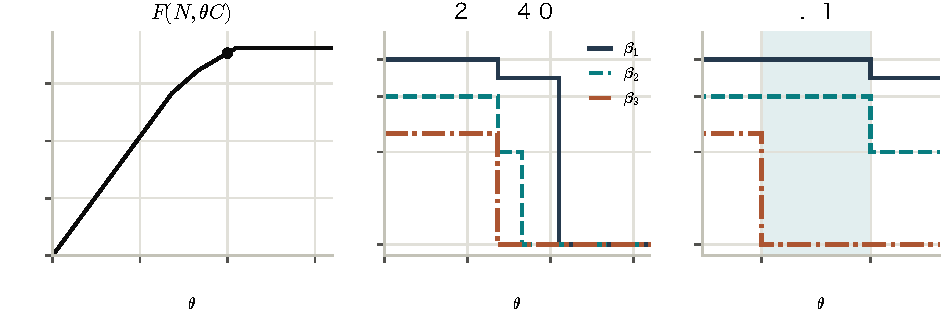
\includegraphics[width=\linewidth]{figures/lp_parametric.pdf}
\caption{库存缩放系数 $\theta$ 下的离线最优值 $F(N,\theta C)$（左）与库存影子价格 $\beta_j(\theta)$（右），$N=(50,30,20)$。竖线为课程实例 $\theta=1$}
\label{fig:parametric}
\end{figure}

\section{问题三：基于库存机会成本的在线推荐策略}\label{sec:policy}

\subsection{设计思路：从离线模型到在线评分}
在线决策的难点在于当期推荐与未来库存之间的权衡。设第 $t$ 期顾客类型为 $i$、库存为 $c$，若已知第 $t+1$ 期起的最优价值函数 $V_{t+1}(\cdot)$，推荐集合 $S$ 的期望总价值为
\begin{equation}
\sum_{j\in S}p_{ij}\bigl[r_j+V_{t+1}(c-e_j)\bigr]+\Bigl(1-\sum_{j\in S}p_{ij}\Bigr)V_{t+1}(c)
=V_{t+1}(c)+\sum_{j\in S}p_{ij}\bigl[r_j-\theta_j\bigr],
\label{eq:lookahead}
\end{equation}
其中 $\theta_j=V_{t+1}(c)-V_{t+1}(c-e_j)$ 是一件商品 $j$ 的机会成本。式\eqref{eq:lookahead}的最优集合由评分 $p_{ij}(r_j-\theta_j)$ 最高、且评分非负的至多 $K$ 件有货商品组成。动态规划可以给出精确的 $\theta_j$，但其状态数为 $\prod_j(C_j+1)$，商品数增加时无法求解。

问题二的离线模型提供了一个可扩展的近似。第 $t$ 期之后还有 $\tau=T-t$ 位顾客，预计各类型人数为 $\tau\lambda$，用剩余销售期的流体线性规划 $F(\tau\lambda,c)$ 近似 $V_{t+1}(c)$，机会成本有两种计算方式：
\begin{align}
\text{对偶价格：}\quad &\theta_j=\beta_j(\tau\lambda,c),\ \text{即 }F(\tau\lambda,c)\text{ 中库存约束 }j\text{ 的对偶变量}; \label{eq:theta_dual}\\
\text{有限差分：}\quad &\theta_j=\Delta_j(\tau\lambda,c)=F(\tau\lambda,c)-F(\tau\lambda,c-e_j). \label{eq:theta_fd}
\end{align}
相应得到两种策略：\LPDual{} 每期求解一个线性规划并读取对偶价格；\LPFD{} 每期求解至多 $n+1$ 个线性规划，按式\eqref{eq:lookahead}做精确的一步前瞻。二者都在每期以最新库存重新求解离线模型，属于收益管理中的投标价格（bid-price）控制与滚动重优化\cite{talluri98,jasin,bumpensanti}。库存感知贪心 \Greedy{} 对应 $\theta=0$，即完全忽略未来。第\ref{sec:exp}节的精确评价表明，\LPDual{} 在五份数据上的期望遗憾低于 \LPFD{} 与 \Greedy{}，本文以 \LPDual{} 作为主策略，\LPFD{} 作为对照。

\subsection{机会成本的性质}
两种机会成本之间存在确定的大小关系。

\begin{proposition}\label{prop:order}
设 $\tau\ge1$，商品 $j$ 满足 $1\le c_j\le\tau$，$\beta$ 为 $F(\tau\lambda,c)$ 的任一最优对偶解，则
\begin{equation}
0\le\beta_j\le\Delta_j\le r_j.
\label{eq:order}
\end{equation}
\end{proposition}
\begin{proof}
$\beta_j\ge0$ 来自对偶可行性。记 $\mu,\nu$ 为其余约束的最优对偶变量，在库存为 $c-e_j$ 的线性规划中，$(\beta,\mu,\nu)$ 仍然对偶可行，由弱对偶得 $F(\tau\lambda,c-e_j)\le F(\tau\lambda,c)-\beta_j$，即 $\beta_j\le\Delta_j$。另一方面，取库存为 $c$ 时的一个最优解 $y$；若商品 $j$ 的期望销量超过 $c_j-1$，按比例缩小各 $y_{ij}$，使其期望销量降为 $c_j-1$。销量至多减少一件，收入至多减少 $r_j$，其余约束仍然满足，故 $F(\tau\lambda,c-e_j)\ge F(\tau\lambda,c)-r_j$，即 $\Delta_j\le r_j$。
\end{proof}

由于每期至多售出一件，$c_j>\tau$ 时商品 $j$ 在剩余期内不会售罄，可以把库存截断为 $\min\{c_j,\tau\}$ 后再求解，此时 $\Delta_j=0$。命题\ref{prop:order}说明，三种策略对稀缺商品的保守程度依次为 $\Greedy<\LPDual\le\LPFD$。$F(\tau\lambda,\cdot)$ 是分段线性凹函数，$\beta_j$ 是当前库存处的局部斜率，$\Delta_j$ 是向左一个单位区间上的平均斜率。在斜率发生跳变的位置附近，有限差分会提前计入下一段更高的边际价值。

\subsection{算法}
算法\ref{alg:dual}给出主策略 \LPDual{} 的完整步骤。离线模型\eqref{eq:lp}只在开始时建立一次，此后每期只修改约束右端项与变量上界，可以利用上一期的单纯形基热启动。

\setcounter{algorithm}{1}% the assignment's Algorithm 1 keeps its number
\begin{algorithm}[htbp]
\caption{\LPDual{}：基于线性规划对偶价格的在线 Top-$K$ 推荐}
\label{alg:dual}
\begin{algorithmic}[1]
\Require prices $r$, purchase probabilities $P$, arrival rates $\lambda$, inventory $C$, slots $K$, horizon $T$; customer types $i_1,\ldots,i_T$ revealed one at a time
\Ensure recommendation sets $S_1,\ldots,S_T$, revenue $R$, final inventory $c$
\State $c\gets C$, $R\gets 0$
\State build LP \eqref{eq:lp} once with variables $y_{ij}$ \Comment{later only RHS and bounds change}
\For{$t=1$ \textbf{to} $T$}
  \State observe $i\gets i_t$; \ $\tau\gets T-t$ \Comment{customers after the current one}
  \If{$\tau=0$}
    \State $\theta\gets 0$
  \Else
    \State $c^{\tau}_j\gets\min\{c_j,\tau\}$ for all $j$
    \State solve $F(\tau\lambda,c^{\tau})$; \ $\theta\gets\beta$ \Comment{duals of the inventory rows}
  \EndIf
  \State $E\gets\{\,j\in A(c):\ p_{ij}r_j>0,\ \ s_j:=p_{ij}(r_j-\theta_j)\ge 0\,\}$
  \State sort $E$ by $s_j$ (descending), then $p_{ij}r_j$ (descending), then $j$ (ascending)
  \State $S_t\gets$ first $\min\{K,|E|\}$ products of $E$
  \State show $S_t$ to the customer and observe the purchase $J'_t\in S_t\cup\{0\}$
  \If{$J'_t=j\neq0$}
    \State $c_j\gets c_j-1$, \ $R\gets R+r_j$
  \EndIf
\EndFor
\State \Return $(S_t)_{t=1}^{T}$, $R$, $c$
\end{algorithmic}
\end{algorithm}

\textbf{对照策略 \LPFD{}。} 把算法\ref{alg:dual}第 9 行替换为
\begin{equation*}
\textbf{for } j\in A(c)\textbf{ do }\ \theta_j\gets F(\tau\lambda,c^{\tau})-F\bigl(\tau\lambda,(c-e_j)^{\tau}\bigr)\ \textbf{end for},
\end{equation*}
其余步骤不变。

\textbf{剩余人数预测 \LPCount{}。} 若平台事先知道整个销售期各类型的总人数 $N$（例如题目给出的五份数据均为 $(50,30,20)$），可以把算法\ref{alg:dual}中的 $\tau\lambda$ 替换为剩余人数的预测
\begin{equation}
d_t=\frac{\tau}{\sum_k(N_k-n_{tk})^+}\,(N-n_t)^+,
\label{eq:countforecast}
\end{equation}
其中 $n_{tk}$ 为前 $t$ 期（含当期）已到达的类型 $k$ 顾客人数。$d_t$ 只用到已观察到的到达和总人数，不使用未来顾客的到达顺序。第\ref{sec:order}节用它衡量到达顺序信息的价值。

\textbf{评分规则的细节。} 第 11 行要求 $p_{ij}r_j>0$，从而购买概率为零的商品不会占用推荐位。评分等于零的商品仍可进入推荐列表：机会成本等于价格时，推荐该商品与空出推荐位的近似价值相同，而前者在库存最终未被占用时还能带来收入。评分相同时优先即时收益较高的商品，再按编号排序，因此策略是状态的确定性函数。比较评分前把数值舍入到 $10^{-9}$，以消除单纯形求解的浮点误差。需要指出，评分并列并非偶然：由互补松弛条件，流体最优解中被同一类顾客混合使用的推荐集合，其调整后收益必然相等。例如 $\beta^{*}=(9,0,0)$ 时，类型 1 顾客对商品 1 与商品 3 的评分都等于 $0.6$。并列规则因此是策略的实质组成部分，第\ref{sec:sens}节讨论它的影响。

\subsection{可行性与计算量}
\begin{proposition}\label{prop:feasible}
对任意到达序列与购买结果，算法\ref{alg:dual}及其两个变体满足：(i) $S_t\subseteq A(c_t)$，$|S_t|\le K$；(ii) 对所有 $t$ 有 $c_t\ge0$，且 $R=\sum_jr_j(C_j-c_{T+1,j})$；(iii) $S_t$ 只依赖 $(i_1,\ldots,i_t)$、$c_t$ 与已实现的购买结果。
\end{proposition}
\begin{proof}
第 11 行只从 $A(c)$ 中选取商品，第 13 行至多取 $K$ 件，得到 (i)。初始库存非负，每期至多售出一件且只售出有货商品，由归纳法得到 (ii)。算法使用的量为 $i_t$、$c_t$、$\tau$ 与固定参数，\LPCount{} 另外使用已观察到的人数 $n_t$，得到 (iii)。
\end{proof}

命题\ref{prop:feasible}对应题目评分中的可行性要求：零缺货推荐，并且可以在不同的 $m,n,T,K$ 下运行。每期的计算量为一次线性规划求解（$mn$ 个变量、$m+n$ 条约束）加上 $O(n\log n)$ 的排序，与库存数量无关，满足题目“不在每一期求解整数规划”的提示。实现中，库存截断后相同的状态会重复出现，程序以 $(\tau,c^{\tau})$ 为键缓存线性规划的结果。缓存只是计算上的加速，不改变策略。第\ref{sec:scale}节报告了不同规模下的单期决策时间。

\subsection{策略在课程实例上的行为}\label{sec:behavior}
以第 1 期为例，$\tau=99$，$F(99\lambda,C)=702.54$，对偶价格 $\beta=(9,0,0)$。三类顾客的评分为
\begin{equation*}
s_{1\cdot}=(0.6,\ 1.6,\ 0.6),\qquad s_{2\cdot}=(0.4,\ 4.0,\ 0),\qquad s_{3\cdot}=(0.1,\ 1.6,\ 3.6).
\end{equation*}
类型 1 的商品 1 与商品 3 评分相同，按即时收益 $6>0.6$ 选择商品 1，三类顾客的推荐集合依次为 $\{1,2\}$、$\{1,2\}$、$\{2,3\}$，与算法 1 相同。$\beta_1=9$ 恰好使类型 1 顾客在商品 1 与商品 3 之间无差异，与第\ref{sec:q2}节“让一位类型 1 顾客把商品 1 换成商品 3、每节省一件商品 1 损失 9”的计算一致。

策略与算法 1 的差别出现在商品 1 变得稀缺之后。商品 2、3 库存充裕时，剩余 $\tau$ 期内类型 2 对商品 1 的流体需求为 $0.3\times0.4\,\tau=0.12\tau$。当 $c_1<0.12\tau$ 时，即使类型 1 完全不买商品 1，类型 2 的需求也会超过库存，此时 $\beta_1=10$，类型 1 顾客的商品 1 评分降为 $0$，低于商品 3 的 $0.6$，商品 1 不再推荐给类型 1，库存留给没有替代选择的类型 2 顾客。记
\begin{equation}
\bar c_1(H)=\max\bigl\{c_1\ge1:\ \text{剩余 }H\text{ 期、}c_2=35,\ c_3=25\text{ 时，类型 1 顾客的推荐集合不含商品 1}\bigr\}
\label{eq:threshold}
\end{equation}
为预留阈值（不存在时取 0）。图\ref{fig:threshold}比较了三种策略的预留阈值：\LPDual{} 的阈值约为 $\lfloor0.12(H-1)\rfloor$，\LPFD{} 约多一件。\IIDDP{} 的阈值约为 \LPDual{} 的两倍，因为随机需求的波动使商品 1 在库存略高于流体需求时仍有较大的售罄概率，动态规划为此保留安全库存。

\begin{figure}[htbp]
\centering
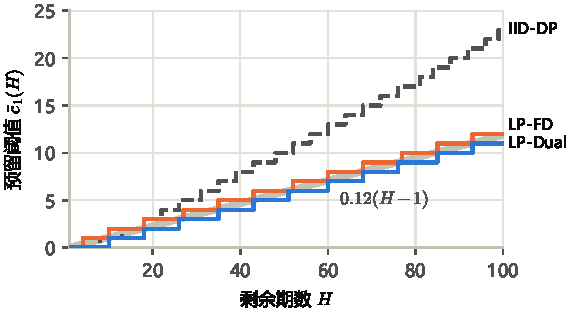
\includegraphics[width=0.64\linewidth]{figures/threshold.pdf}
\caption{预留阈值 $\bar c_1(H)$：库存不超过该值时，类型 1 顾客不再看到商品 1（$c_2=35$，$c_3=25$）。灰线为类型 2 对商品 1 的流体需求 $0.12(H-1)$}
\label{fig:threshold}
\end{figure}

\LPFD{} 的阈值更高，原因在于有限差分在销售期末尾高估最后几件库存的价值。取 $c_1=1$，商品 2、3 充裕，剩余 $\tau$ 期内商品 1 的总流体需求为 $(0.5\times0.6+0.3\times0.4)\tau=0.42\tau$，其中类型 2 的需求为 $0.12\tau$。当 $3\le\tau\le8$ 时 $0.12\tau<1<0.42\tau$，$F(\tau\lambda,\cdot)$ 关于 $c_1$ 在 $[0,0.12\tau]$ 上的斜率为 10（每件都能卖给没有替代选择的类型 2），在 $[0.12\tau,\,1]$ 上的斜率为 9，于是
\begin{equation}
\beta_1=9,\qquad \Delta_1=10\times0.12\tau+9\times(1-0.12\tau)=9+0.12\tau>\beta_1.
\label{eq:fdend}
\end{equation}
类型 1 顾客的商品 1 评分 $0.6(1-0.12\tau)$ 低于商品 3 的 $0.6$，\LPFD{} 不再向类型 1 推荐最后一件商品 1；\LPDual{} 的两件商品评分相等，按即时收益推荐商品 1。真实情况是，剩余 $\tau$ 期内出现一位想买商品 1 的类型 2 顾客的概率为 $1-0.88^{\tau}$，$\tau=5$ 时只有 $47\%$。\LPFD{} 为它保留的最后一件商品 1 常常到期末仍未售出。（$\tau\le2$ 时总流体需求 $0.42\tau<1$，商品 1 不再稀缺，$\beta_1=0$，而 $\Delta_1=3.9\tau$ 仍为正数，\LPFD{} 同样偏保守。）第\ref{sec:where}节用精确的损失分解验证这一机制。

\section{评价方法}\label{sec:eval}
本节给出三类工具：两种动态规划基准、无蒙特卡洛误差的精确策略评价，以及蒙特卡洛模拟的统计量。后两者分别用于计算期望遗憾和刻画单次实现的波动。

\subsection{两种动态规划基准}
\textbf{序列已知的动态规划（\SeqDP）。} 固定到达序列 $i_{1:T}$，以 $V_t(c)$ 表示第 $t$ 期开始、库存为 $c$ 时的最优期望收入，$V_{T+1}(c)=0$，Bellman 方程为
\begin{equation}
V_t(c)=V_{t+1}(c)+\max_{\substack{S\subseteq A(c)\\|S|\le K}}\ \sum_{j\in S}p_{i_tj}\bigl[r_j+V_{t+1}(c-e_j)-V_{t+1}(c)\bigr].
\label{eq:seqdp}
\end{equation}
记 $V^{\seq}=V_1(C)$。\SeqDP{} 预先知道全部顾客类型，购买结果仍然随机，它给出了任何在线策略在该序列上所能达到的期望收入上限，满足 $\E[R_T(\pi)\mid i_{1:T}]\le V^{\seq}\le F(N,C)$。\SeqDP{} 使用了未来信息，只作为诊断基准。

\textbf{独立同分布到达下的动态规划（\IIDDP）。} 若后续顾客类型按 $\lambda$ 独立到达，以 $W_h(c)$ 表示剩余 $h$ 期、尚未观察下一位顾客时的最优价值，$W_0(c)=0$，
\begin{equation}
W_h(c)=\sum_{i=1}^{m}\lambda_i\Bigl[W_{h-1}(c)+\max_{\substack{S\subseteq A(c)\\|S|\le K}}\ \sum_{j\in S}p_{ij}\bigl[r_j+W_{h-1}(c-e_j)-W_{h-1}(c)\bigr]\Bigr].
\label{eq:iiddp}
\end{equation}
把每个 $(h,i,c)$ 上的最优动作存成表格，就得到一个在线策略 \IIDDP{}：它只使用 $\lambda$ 与当前状态，在独立同分布到达下是最优在线策略。课程实例的库存状态共 $41\times36\times26=38{,}376$ 个，100 期、3 类顾客的动作表含约 1150 万项，向量化递推用时约 \IIDSeconds{} 秒。状态数随商品数按 $\prod_j(C_j+1)$ 指数增长，动态规划因而只适合作为小规模实例上的基准；线性规划策略的规模为 $mn$，可以扩展到更大的问题。

\subsection{精确策略评价}\label{sec:exact}
本文比较的策略都在第 $t$ 期依据 $(t,i_t,c_t)$ 选择推荐集合，记为 $S_t(c)$。给定到达序列后，库存过程是格点 $\mathcal L=\prod_j\{0,1,\ldots,C_j\}$ 上的非齐次马尔可夫链。令 $D_t(c)=\Pr(c_t=c)$，$D_1$ 集中在 $C$ 上，则
\begin{equation}
D_{t+1}(c)=D_t(c)\Bigl(1-\sum_{j\in S_t(c)\cap A(c)}p_{i_tj}\Bigr)+\sum_{j=1}^{n}D_t(c+e_j)\,p_{i_tj}\,\ind\bigl\{j\in S_t(c+e_j)\bigr\}.
\label{eq:forward}
\end{equation}
式中 $S_t(c)\cap A(c)$ 剔除了缺货商品，可以同时处理会推荐缺货商品的算法 1。收入由期末库存唯一决定：
\begin{equation}
R_T=\sum_{j=1}^{n}r_j\bigl(C_j-c_{T+1,j}\bigr),
\label{eq:revenue}
\end{equation}
因此 $D_{T+1}$ 直接给出 $R_T$ 的精确分布，进而得到期望收入、标准差、$\Pr(R_T>F)$、期望剩余库存 $\E c_{T+1,j}$ 与售罄概率 $q_j=\Pr(c_{T+1,j}=0)$。每一步递推的计算量为 $O(n|\mathcal L|)$，课程实例上一条序列的全部递推约需 \ExactSeconds{} 秒。

两种 LP 策略的动作依赖 $F(\tau\lambda,c)$ 在整个格点上的取值。由于每期至多售出一件，库存超过剩余期数 $\tau$ 的部分不会形成约束，求解时可以把 $c_j$ 截断为 $\min\{c_j,\tau\}$。本文对 $\tau=0,\ldots,99$ 与全部截断状态共求解约 283 万个线性规划（14 个进程并行，用时 \TableSeconds{} 秒），然后生成每个 $(h,i,c)$ 的动作表。在五份数据各 300 条模拟路径上，两种策略共 \VerifyDecisions{} 次决策中，动作表与在线策略对象给出的推荐集合不一致的次数为 \VerifyMismatch{}；单元测试还在缩小的实例上把式\eqref{eq:forward}的结果与逐状态枚举、后向递推进行了对照。

\subsection{遗憾分解}
对固定序列 $s$，期望遗憾可以分解为
\begin{equation}
G_s(\pi)=F_s-\E[R_T(\pi)\mid s]=\underbrace{F_s-V_s^{\seq}}_{\text{流体松弛间隙}}+\underbrace{V_s^{\seq}-\E[R_T(\pi)\mid s]}_{\text{策略损失}}.
\label{eq:gap}
\end{equation}
记 $L_s(\pi)=V_s^{\seq}-\E[R_T(\pi)\mid s]\ge0$ 为策略损失。流体松弛间隙与策略无关：流体模型用期望销量代替随机销量，库存约束只在期望意义下成立；随机需求低于库存时余量无法转移给其他时段，高于库存时多余需求流失，由 Jensen 不等式 $\E\min\{D,C\}\le\min\{\E D,C\}$，随机系统的可达收入低于流体值。策略损失衡量在线策略与预知顾客类型的最优策略之间的差距，其中包含不知道未来到达顺序的代价。任何在线策略都无法消除流体松弛间隙，比较策略时应关注 $L_s(\pi)$。

\subsection{蒙特卡洛统计量}\label{sec:mc}
对序列 $s$ 的第 $b$ 次重复，各策略共享同一组潜在首选 $J_{1:T}^{(s,b)}$。记策略 $\pi$ 的收入为 $R^{\pi}_{sb}$，$b=1,\ldots,B$，定义
\begin{equation}
\overline R_s^{\pi}=\frac1B\sum_{b=1}^{B}R^{\pi}_{sb},\qquad
h_s^{\pi}=t_{0.975,B-1}\frac{\hat\sigma_s^{\pi}}{\sqrt B},\qquad
\bar d_s^{\,\pi\pi'}=\frac1B\sum_{b=1}^{B}\bigl(R^{\pi}_{sb}-R^{\pi'}_{sb}\bigr),
\label{eq:mcstats}
\end{equation}
其中 $\hat\sigma_s^{\pi}$ 为样本标准差，$h_s^{\pi}$ 是 95\% 置信区间的半宽；配对差 $\bar d_s^{\,\pi\pi'}$ 的半宽 $h_s^{\,\pi\pi'}$ 按同一公式由逐次差值的样本标准差计算。主实验取 $B=2000$，随机种子为 20261107，五份数据使用独立的随机流。

\section{数值实验}\label{sec:exp}

\subsection{实验设计}\label{sec:design}
表\ref{tab:policies}列出参与比较的策略。前五种是在线策略，\SeqDP{} 预知整条类型序列，只作为策略损失的基准。所有策略在全部实验中使用相同的规则与参数，没有针对任何数据集调整。

\begin{table}[htbp]
\centering\small
\caption{参与比较的策略}\label{tab:policies}
\begin{tabularx}{\linewidth}{@{}l X l l@{}}
\toprule
策略 & 推荐规则 & 决策所用信息 & 每期计算\\
\midrule
\AlgOne{} & 题目算法 1：按 $v_{ij}$ 固定推荐前 $K$ 件，不检查库存 & $i_t$ & 无\\
\Greedy{} & 在有货商品中按 $v_{ij}$ 推荐前 $K$ 件 & $i_t,\ c_t$ & 排序\\
\LPDual{} & 算法\ref{alg:dual}，机会成本取对偶价格\eqref{eq:theta_dual} & $i_t,\ c_t,\ \tau,\ \lambda$ & 1 个 LP\\
\LPFD{} & 算法\ref{alg:dual}，机会成本取有限差分\eqref{eq:theta_fd} & $i_t,\ c_t,\ \tau,\ \lambda$ & $\le n+1$ 个 LP\\
\LPCount{} & \LPDual{}，需求预测改用剩余人数\eqref{eq:countforecast} & $i_t,\ c_t,\ n_t,\ N$ & 1 个 LP\\
\IIDDP{} & 式\eqref{eq:iiddp}的最优动作表 & $i_t,\ c_t,\ \tau,\ \lambda$ & 查表\\
\SeqDP{} & 式\eqref{eq:seqdp}的最优动作，预知 $i_{1:T}$ & $i_{1:T},\ c_t$ & 基准\\
\bottomrule
\end{tabularx}
\end{table}

实验分为六组：
\begin{enumerate}[label=(\arabic*)]
\item 题目给出的五份数据：精确评价各策略，并对每份数据做 $B=2000$ 次蒙特卡洛重复（第\ref{sec:main}--\ref{sec:where}节）；
\item 1000 条生成序列：500 条人数为 $(50,30,20)$ 的随机排列，500 条按 $\lambda$ 独立同分布生成的序列（第\ref{sec:random}节）；
\item 六种分块到达顺序，检验需求预测失准时的表现（第\ref{sec:order}节）；
\item 库存缩放 $\theta\in\{0.3,0.4,\ldots,1.2\}$ 与推荐位数 $K\in\{1,2,3\}$（第\ref{sec:sens}节）；
\item 销售期 $T$ 从 25 增至 1600、库存同比例放大（第\ref{sec:scale}节）；
\item 随机生成的较大实例，最大为 $(m,n,T,K)=(20,30,300,4)$（第\ref{sec:scale}节）。
\end{enumerate}
第 (1)--(4) 组的期望值均由第\ref{sec:exact}节的方法精确计算，第 (5)、(6) 组的状态空间过大，采用蒙特卡洛模拟。计算环境为 Python 3.11.9、Gurobi 13.0.3（单线程对偶单纯形法）、NumPy 1.26.4。

\subsection{五份数据上的结果}\label{sec:main}
表\ref{tab:main}给出主策略 \LPDual{} 的逐份结果，表\ref{tab:aggregate}汇总各策略的表现。\LPDual{} 在五份数据上的平均期望收入为 \ERDual{}，达到离线上界 706 的 \RatioDual\%；平均遗憾 $\overline G=\GavgDual$，最大遗憾 $G_{\max}=\GmaxDual$，全部推荐满足库存约束。期末平均剩余商品 1 \EconeDual{} 件、商品 2 \EctwoDual{} 件、商品 3 \EcthreeDual{} 件，商品 1 在 \SoldOutEndDual\% 的路径上售罄。商品 2、3 的剩余量与流体解的剩余量 $\bar c=(0,\,6,\,38/3)$ 接近，说明商品 2、3 本身库存充裕，剩余是需求不足的自然结果；商品 1 是唯一的稀缺商品。

\begin{table}[htbp]
\centering\small
\caption{\LPDual{} 在五份数据上的期望结果与首次模拟}\label{tab:main}
\begin{tabular}{lrrrrrr}
\toprule
指标 & D1 & D2 & D3 & D4 & D5 & 五组均值 \\
\midrule
\multicolumn{7}{l}{\textit{固定到达序列，对购买结果取期望}} \\
期望收入 $\E R_T$ & 695.854 & 696.397 & 695.260 & 696.130 & 695.827 & 695.894 \\
期望遗憾 $G_s$ & 10.146 & 9.603 & 10.740 & 9.870 & 10.173 & 10.106 \\
策略损失 $L_s$ & 0.099 & 0.090 & 0.215 & 0.225 & 0.214 & 0.169 \\
商品 1 期末库存 & 0.907 & 0.894 & 0.905 & 0.897 & 0.912 & 0.903 \\
商品 2 期末库存 & 6.177 & 6.183 & 6.175 & 6.179 & 6.175 & 6.178 \\
商品 3 期末库存 & 12.610 & 12.533 & 12.716 & 12.579 & 12.608 & 12.609 \\
商品 1 售罄概率 & 70.8\% & 71.9\% & 71.6\% & 71.8\% & 71.7\% & 71.6\% \\
\midrule
模拟均值 $\overline R_s$ & 696.237 & 697.303 & 695.309 & 695.564 & 695.891 & 696.061 \\
95\% 区间半宽 $h_s$ & 1.250 & 1.230 & 1.234 & 1.216 & 1.248 & -- \\
\midrule
\multicolumn{7}{l}{\textit{每份数据的首次购买模拟}} \\
实现收入 $R_T^{(1)}$ & 678 & 710 & 680 & 660 & 656 & 676.8 \\
实现遗憾 $F_s-R_T^{(1)}$ & 28 & -4 & 26 & 46 & 50 & 29.2 \\
期末库存 & $(0,10,12)$ & $(0,3,16)$ & $(5,2,14)$ & $(0,13,11)$ & $(0,12,13)$ & -- \\
\bottomrule
\end{tabular}
\par\vspace{0.35em}{\footnotesize 五份数据的 $F_s$ 均为 706。期望值和售罄概率由精确递推得到。每份数据的首次模拟均使用预设随机流的首组购买抽样，五条路径共出现 \FirstOosSlots{} 次缺货推荐。期望遗憾的最大值为 \GmaxDual，首次模拟的最大实现遗憾为 \FirstMaxRegret。}
\end{table}

\begin{table}[htbp]
\centering\small
\caption{各策略在五份数据上的综合表现}\label{tab:aggregate}
\begin{tabular}{lrrrrrr}
\toprule
策略 & $\overline{\E R_T}$ & $\overline G$ & $G_{\max}$ & $\overline G^{\,\mathrm{MC}}$ & $\overline L$ & $\overline W$ \\
\midrule
\AlgOne{} & 693.394 & 12.606 & 12.606 & 12.426 & 2.669 & 6.29 \\
\Greedy{} & 695.550 & 10.450 & 11.168 & 10.318 & 0.513 & 0.00 \\
\LPFD{} & 695.490 & 10.510 & 11.058 & 10.306 & 0.572 & 0.00 \\
\LPDual{} & 695.894 & 10.106 & 10.740 & 9.939 & 0.169 & 0.00 \\
\LPCount{} & 695.768 & 10.232 & 11.147 & 10.121 & 0.295 & 0.00 \\
\IIDDP{} & 695.862 & 10.138 & 10.815 & 9.995 & 0.201 & 0.00 \\
\SeqDP{} & 696.062 & 9.938 & 10.525 & -- & 0.000 & -- \\
\bottomrule
\end{tabular}
\par\vspace{0.35em}{\footnotesize $\overline G$ 与 $G_{\max}$ 按式\eqref{eq:avgmax}由精确期望计算；$\overline G^{\,\mathrm{MC}}=\frac15\sum_s(F_s-\overline R_s)$ 为模拟估计；$\overline L$ 为五份数据上策略损失 $L_s$ 的平均；$\overline W$ 为每条路径上缺货推荐的期望次数，定义见式\eqref{eq:waste}。\LPCount{} 使用了总人数 $N$；\SeqDP{} 预知顾客类型序列，只作为基准。}
\end{table}


与其他策略相比：
\begin{itemize}
\item \LPDual{} 在全部五份数据上都高于 \Greedy{}，期望收入差为 \DualGreedyMin--\DualGreedyMax；在 \DualFDWins{} 份数据上高于 \LPFD{}，平均高 \DualFDAvg。
\item \IIDDP{} 是独立同分布到达假设下的最优在线策略，在五份数据上的平均期望收入为 \ERIID{}。它在 4 份数据上高于 \LPDual{}（差距不超过 0.22），但在数据 1 上低 0.67，平均因而略低于 \LPDual{}。\IIDDP{} 为后段可能到来的类型 2 顾客保留安全库存（预留阈值约为 \LPDual{} 的两倍，见图\ref{fig:threshold}）。数据 1 的第 91--93 期连续到达 3 位类型 1 顾客，\IIDDP{} 不向他们推荐商品 1，而第 94--100 期只有 3 位类型 2 顾客，保留的商品 1 有一部分没能售出：它在数据 1 上的策略损失有 99\% 属于多留，集中在第 92、93 期，期末商品 1 的售罄概率只有 58\%，\SeqDP{} 为 72\%。第\ref{sec:random}节的 1000 条生成序列上，\IIDDP{} 平均更优，五份数据上的平均排序受数据 1 影响。
\item \SeqDP{} 的平均期望收入为 \ERSeq，是任何在线策略在这五份数据上的上限。\LPDual{} 的平均策略损失为 \LavgDual，即使预知全部顾客类型，期望收入也只能再提高这么多。
\item 算法 1 在五份数据上的期望收入都是 \AlgOneER{}，平均每条路径出现 \AlgOneOOS{} 次缺货推荐，比 \Greedy{} 低 \AlgOneLossGreedy。
\end{itemize}

模拟结果与精确值吻合：五种可模拟策略在五份数据上的 \MCtotal{} 个模拟均值中，有 \MCinside{} 个落在精确值的 95\% 置信区间内，标准化偏差 $|\overline R_s-\E R_T|\sqrt B/\hat\sigma_s$ 的最大值为 \MCmaxZ。需要注意，$B=2000$ 时单个策略的置信区间半宽约为 \MChw，大于策略之间 0.3--0.9 的期望收入差异，仅凭模拟均值无法可靠地给策略排序。公共随机数大幅降低了配对比较的方差：\LPDual{} 与 \Greedy{} 在 \MCpairEqual\% 的重复中收入完全相同，配对差的半宽只有约 \MCpairhw。精确评价彻底消除了这一不确定性。图\ref{fig:mainloss}按数据集给出四种策略的策略损失。

\begin{figure}[htbp]
\centering
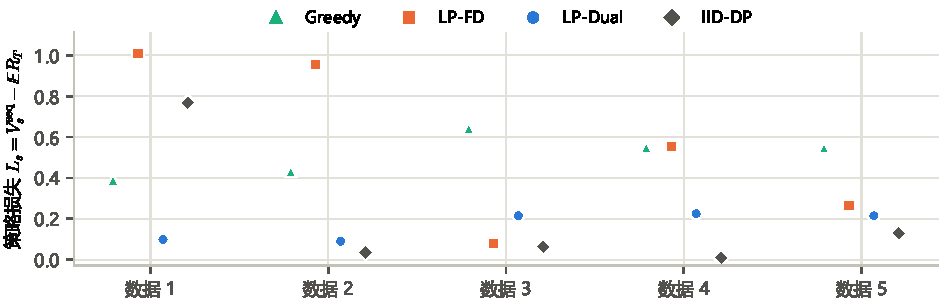
\includegraphics[width=\linewidth]{figures/main_loss.pdf}
\caption{五份数据上各策略的策略损失 $L_s=V^{\seq}_s-\E R_T$（精确值）}
\label{fig:mainloss}
\end{figure}

\subsection{遗憾的构成}\label{sec:decomp}
按式\eqref{eq:gap}分解，五份数据的流体松弛间隙 $F_s-V^{\seq}_s$ 介于 \FluidGapMin{} 与 \FluidGapMax{} 之间，平均为 \FluidGap，占 \LPDual{} 平均遗憾的 \FluidShare\%。换言之，\LPDual{} 的遗憾几乎全部来自流体模型与随机系统之间的差异，在线决策本身造成的损失只有 \LavgDual。

由于 $R_T=\sum_jr_j(C_j-c_{T+1,j})$ 且 $F=\sum_jr_js^{*}_j$（$s^{*}=(40,29,37/3)$ 为流体最优销量），期望遗憾可以按商品精确分解：
\begin{equation}
G_s=\sum_{j=1}^{n}\delta_j,\qquad \delta_j=r_j\bigl(\E c_{T+1,j}-\bar c_j\bigr),\qquad \bar c_j=C_j-s^{*}_j,
\label{eq:productgap}
\end{equation}
其中 $\bar c=(0,\,6,\,38/3)$ 是流体解的剩余库存，$\delta_j$ 是商品 $j$ 比流体解多剩下的库存所对应的收入。表\ref{tab:product}显示，\LPDual{} 的遗憾中有 \ContribOneDual（\ContribOneShare\%）来自商品 1 的剩余。流体解恰好卖完 40 件商品 1，随机系统做不到这一点。若每位类型 1、2 顾客都看到商品 1，商品 1 的潜在购买次数 $D_1=\mathrm{Bin}(50,0.6)+\mathrm{Bin}(30,0.4)$ 的均值为 42、标准差为 \DemandOneSd，$\Pr(D_1<40)=\DemandOneShort\%$，$\E(40-D_1)^+=\DemandOneLeft$。也就是说，即使从不预留商品 1，期末平均仍会剩下约 0.92 件，对应约 9.2 的收入。这部分剩余由需求的随机性决定，预知顾客类型的 \SeqDP{} 也剩下 \EconeSeq{} 件。

\begin{table}[htbp]
\centering\small
\caption{按商品分解的期望遗憾（五份数据平均），$\delta_j$ 的定义见式\eqref{eq:productgap}}\label{tab:product}
\begin{tabular}{lrrrrrrr}
\toprule
策略 & $\E c_{T+1,1}$ & $\E c_{T+1,2}$ & $\E c_{T+1,3}$ & $\delta_1$ & $\delta_2$ & $\delta_3$ & $\overline G=\sum_j\delta_j$ \\
\midrule
\AlgOne{} & 0.923 & 6.172 & 13.000 & 9.228 & 1.378 & 2.000 & 12.606 \\
\Greedy{} & 0.911 & 6.172 & 12.660 & 9.113 & 1.378 & -0.040 & 10.450 \\
\LPFD{} & 0.987 & 6.194 & 12.514 & 9.871 & 1.552 & -0.914 & 10.510 \\
\LPDual{} & 0.903 & 6.178 & 12.609 & 9.029 & 1.423 & -0.346 & 10.106 \\
\IIDDP{} & 0.935 & 6.185 & 12.552 & 9.351 & 1.476 & -0.688 & 10.138 \\
\SeqDP{} & 0.904 & 6.188 & 12.566 & 9.037 & 1.507 & -0.607 & 9.938 \\
\bottomrule
\end{tabular}
\end{table}


收入的随机波动远大于策略间的差异。图\ref{fig:dist}给出 \LPDual{} 在数据 1 上的精确收入分布：标准差约为 \SdDual，单条路径的收入超过 $F=706$ 的概率为 \ProbAboveFDOne\%（五份数据为 \PnegDualMin\%--\PnegDualMax\%），这些路径的样本遗憾为负。题目要求的遗憾若按单次实现计算，主要反映购买结果的运气。本文因此以条件期望 $\E[R_T\mid s]$ 定义 $G_s$，并在表\ref{tab:main}中同时报告模拟均值与置信区间。

\begin{figure}[htbp]
\centering
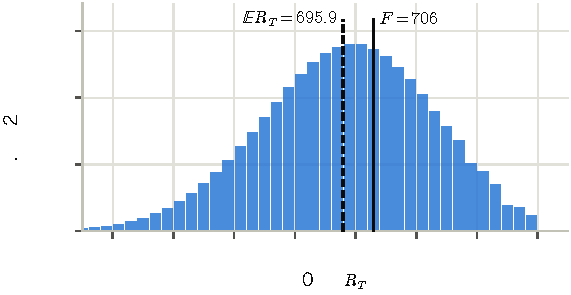
\includegraphics[width=0.66\linewidth]{figures/revenue_dist.pdf}
\caption{\LPDual{} 在数据 1 上的总收入 $R_T$ 的精确分布}
\label{fig:dist}
\end{figure}

\subsection{策略损失的来源}\label{sec:where}
为了定位策略损失，以 \SeqDP{} 的价值函数为尺度评价每一期的决策。令
\begin{equation}
Q_t(c,S)=\sum_{j\in S}p_{i_tj}\bigl[r_j+V_{t+1}(c-e_j)-V_{t+1}(c)\bigr],\qquad Q^{*}_t(c)=\max_{S\subseteq A(c),|S|\le K}Q_t(c,S),
\end{equation}
由 $V_t=V_{t+1}+Q^{*}_t$ 逐期展开，对任意策略 $\pi$ 有
\begin{equation}
L_s(\pi)=\sum_{t=1}^{T}\E_{\pi}\bigl[Q^{*}_t(c_t)-Q_t(c_t,S^{\pi}_t)\bigr],
\label{eq:pdl}
\end{equation}
求和中的每一项都非负，表示第 $t$ 期决策相对最优决策的期望损失，期望按策略 $\pi$ 自身的库存分布计算。本文用第\ref{sec:exact}节的前向递推精确计算式\eqref{eq:pdl}，数值上 $|\sum_t(\cdot)-L_s|\le\LossIdentityErr$。按决策类型，把每一期的损失分为三类：$L^{\mathrm{sell}}$ 为类型 1 顾客看到了最优决策不推荐的商品 1（多卖），$L^{\mathrm{hold}}$ 为类型 1 顾客没有看到最优决策推荐的商品 1（多留），$L^{\mathrm{oth}}$ 为其余决策的损失；再按时段把损失分为 $L_{[1,60]}$、$L_{[61,90]}$、$L_{[91,100]}$。

\begin{table}[htbp]
\centering\small
\caption{策略损失按决策类型与时段的分解（五份数据平均）}\label{tab:loss}
\begin{tabular}{lrrrrrrr}
\toprule
策略 & $\overline L$ & $\overline L^{\mathrm{sell}}$ & $\overline L^{\mathrm{hold}}$ & $\overline L^{\mathrm{oth}}$ & $\overline L_{[1,60]}$ & $\overline L_{[61,90]}$ & $\overline L_{[91,100]}$ \\
\midrule
\Greedy{} & 0.513 & 0.357 & 0.000 & 0.156 & 0.007 & 0.438 & 0.068 \\
\LPFD{} & 0.572 & 0.010 & 0.530 & 0.032 & 0.003 & 0.093 & 0.476 \\
\LPDual{} & 0.169 & 0.112 & 0.010 & 0.046 & 0.003 & 0.099 & 0.067 \\
\IIDDP{} & 0.201 & 0.020 & 0.155 & 0.025 & 0.000 & 0.045 & 0.155 \\
\bottomrule
\end{tabular}
\end{table}


表\ref{tab:loss}与图\ref{fig:losstime}给出三种策略各自的失误模式：
\begin{itemize}
\item \Greedy{} 的主要损失是多卖（\LossSellGreedy）。它对类型 1 顾客始终推荐商品 1，商品 1 售罄得过早：第 80 期结束时，\Greedy{} 下商品 1 已售罄的概率为 \SoldOutEightyGreedy\%，\LPDual{} 为 \SoldOutEightyDual\%，\LPFD{} 与 \IIDDP{} 更低。售罄之后到达的类型 2 顾客没有替代商品可买，损失集中在第 61--90 期（\LossMidGreedy）。
\item \LPFD{} 的总损失为 \LavgFD，主要是多留（\LossHoldFD），时间上集中在最后 10 期（\LossEndFD），与第\ref{sec:behavior}节式\eqref{eq:fdend}的分析一致：有限差分在期末高估最后一件商品 1 的价值，把它留给不一定到来的类型 2 顾客。期末商品 1 的售罄概率只有 \SoldOutEndFD\%，低于 \SeqDP{} 的 \SoldOutEndSeq\%。
\item \LPDual{} 介于两者之间，多卖 \LossSellDual、多留 \LossHoldDual，总损失最小。命题\ref{prop:order}中 $0=\theta^{\Greedy}\le\beta\le\Delta$ 的大小关系，在这里对应 \Greedy{} 偏激进、\LPFD{} 偏保守、\LPDual{} 居中。
\end{itemize}

\begin{figure}[htbp]
\centering
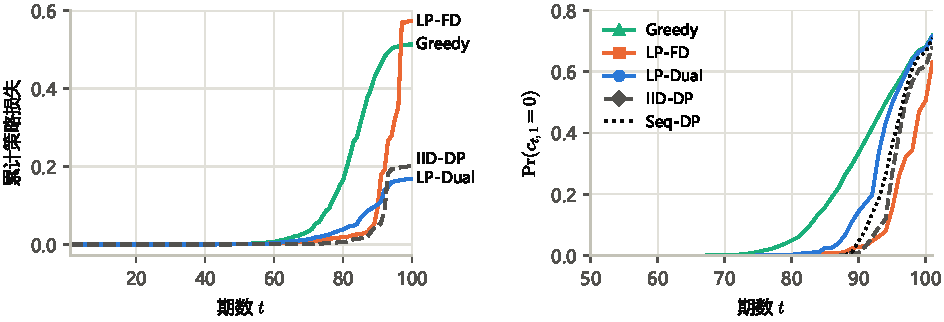
\includegraphics[width=\linewidth]{figures/loss_time.pdf}
\caption{五份数据平均的累计策略损失（左）与商品 1 已售罄的概率 $\Pr(c_{t,1}=0)$（右）}
\label{fig:losstime}
\end{figure}

\subsection{生成序列上的表现}\label{sec:random}
五份给定数据只是众多可能到达顺序中的五个样本。为检验结论是否依赖这五个样本，本文生成了两组序列：500 条人数固定为 $(50,30,20)$ 的随机排列，与给定数据的生成方式相同；500 条按 $\lambda$ 独立同分布生成的序列，各类型人数随机，$F_s$ 介于 \FminIid{} 与 \FmaxIid{} 之间。第\ref{sec:instance}节已说明，五份给定数据可以视为第一组序列的典型样本。表\ref{tab:random}与图\ref{fig:random}给出精确评价的结果。

\begin{table}[htbp]
\centering\small
\caption{生成序列上的精确期望遗憾与策略损失}\label{tab:random}
\begin{tabular}{lrrrrrrrr}
\toprule
 & \multicolumn{4}{c}{随机排列（500 条）} & \multicolumn{4}{c}{独立同分布到达（500 条）} \\
\cmidrule(lr){2-5}\cmidrule(lr){6-9}
策略 & $\overline G$ & $G_{0.95}$ & $G_{\max}$ & $\overline L$ & $\overline G$ & $G_{0.95}$ & $G_{\max}$ & $\overline L$ \\
\midrule
\AlgOne{} & 12.606 & 12.606 & 12.606 & 2.901 & 12.522 & 17.983 & 21.979 & 3.260 \\
\Greedy{} & 10.226 & 10.895 & 11.757 & 0.520 & 9.906 & 16.423 & 18.861 & 0.644 \\
\LPFD{} & 10.200 & 11.099 & 12.927 & 0.495 & 9.711 & 16.331 & 19.674 & 0.449 \\
\LPDual{} & 9.902 & 10.551 & 11.426 & 0.197 & 9.513 & 16.148 & 18.451 & 0.251 \\
\IIDDP{} & 9.801 & 10.421 & 11.044 & 0.096 & 9.370 & 15.987 & 18.207 & 0.108 \\
\bottomrule
\end{tabular}
\par\vspace{0.35em}{\footnotesize $G_{0.95}$ 为 500 条序列上期望遗憾的 95\% 分位数。两组序列的 $F_s$ 与 $V^{\seq}_s$ 逐条计算。}
\end{table}


\begin{figure}[htbp]
\centering
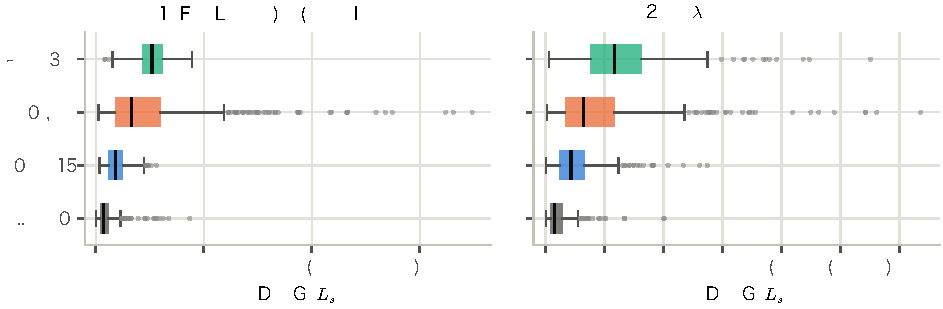
\includegraphics[width=\linewidth]{figures/random.pdf}
\caption{1000 条生成序列上的策略损失分布（箱线图，箱体为四分位区间）}
\label{fig:random}
\end{figure}

随机排列上，\LPDual{} 的平均遗憾为 \GavgDualPerm，低于 \Greedy{} 的 \GavgGreedyPerm{} 与 \LPFD{} 的 \GavgFDPerm{}；它在 \DualBeatsGreedyPerm\% 的序列上不低于 \Greedy{}，在 \DualBeatsFDPerm\% 的序列上不低于 \LPFD{}。\IIDDP{} 的平均策略损失为 \LavgIIDPerm，低于 \LPDual{} 的 \LavgDualPerm，后者在 \DualBeatsIIDPerm\% 的序列上不低于 \IIDDP{}。这一结果符合预期：随机排列接近独立同分布到达，此时 \IIDDP{} 是最优在线策略。\LPDual{} 只需求解规模为 $mn$ 的线性规划，就取得了 \IIDDP{} 的大部分收益。独立同分布序列上的排序相同。

\LPFD{} 的损失分布有一条长尾，最大值为 \LmaxFDPerm，而 \LPDual{} 不超过 \LmaxDualPerm。长尾来自期末的过度预留：\LPFD{} 的策略损失与最后 10 期类型 2 顾客人数的相关系数为 \CorrFDLastTen{}，损失最大的 10 条序列在最后 10 期至多有 \TopFDLastTenMax{} 位类型 2 顾客（期望为 3 位）。\Greedy{} 与 \LPDual{} 的损失则与最后 20 期类型 2 的人数正相关（相关系数分别为 \CorrGreedyLastTwenty{} 与 \CorrDualLastTwenty{}），它们的主要风险是多卖，后段类型 2 顾客越多，越早售罄商品 1 的代价越大。算法 1 的推荐集合只依赖顾客类型，各商品的销量只取决于各类型的人数，与到达顺序无关，因此它在全部 500 条随机排列上的期望收入相同。

\subsection{到达顺序与需求预测}\label{sec:order}
\LPDual{}、\LPFD{} 与 \IIDDP{} 都假设未来顾客按 $\lambda$ 到达。为检验预测失准的后果，本文把三类顾客分块排列，构造六种极端到达顺序，结果见表\ref{tab:order}。

\begin{table}[htbp]
\centering\small
\caption{分块到达顺序下的期望收入}\label{tab:order}
\begin{tabular}{lrrrrrrr}
\toprule
到达顺序 & \Greedy{} & \LPFD{} & \LPDual{} & \LPCount{} & \IIDDP{} & \SeqDP{} & $\E c^{\LPDual}_{T+1,1}$ \\
\midrule
$1\to2\to3$ & 694.050 & 694.200 & 694.199 & 690.984 & 693.735 & 694.543 & 0.851 \\
$1\to3\to2$ & 693.395 & 693.626 & 693.588 & 690.307 & 693.126 & 693.946 & 0.923 \\
$2\to1\to3$ & 696.997 & 674.747 & 683.029 & 696.999 & 670.601 & 697.000 & 2.360 \\
$2\to3\to1$ & 696.806 & 694.261 & 695.511 & 696.782 & 694.757 & 696.812 & 0.830 \\
$3\to1\to2$ & 693.395 & 693.444 & 693.416 & 691.694 & 693.588 & 693.908 & 0.923 \\
$3\to2\to1$ & 696.806 & 696.075 & 696.707 & 696.807 & 696.498 & 696.809 & 0.923 \\
\bottomrule
\end{tabular}
\par\vspace{0.35em}{\footnotesize 表中为精确期望收入，各顺序的 $F_s$ 均为 706。$1\to2\to3$ 表示先到达 50 位类型 1 顾客，再到达 30 位类型 2 与 20 位类型 3 顾客，其余类推。算法 1 在任何顺序下的期望收入都是 \AlgOneER{}。}
\end{table}


顺序 $2\to1\to3$ 下，三种依赖到达率的策略都明显变差：\LPDual{} 为 \BlockDual，\LPFD{} 为 \BlockFD，\IIDDP{} 为 \BlockIID，而 \Greedy{} 达到 \BlockGreedy，与 \SeqDP{} 的 \BlockSeq{} 几乎相同。图\ref{fig:order}显示了原因：第 31--80 期到达的全部是类型 1 顾客，策略仍然预期此后有 30\% 的顾客属于类型 2，按第\ref{sec:behavior}节的预留阈值为它们保留商品 1；实际上第 30 期之后不再有类型 2 顾客，保留的库存最终无人购买。期末商品 1 的期望剩余为 \BlockEconeDual（\LPDual）和 \BlockEconeIID（\IIDDP），\Greedy{} 只剩 \BlockEconeGreedy。损失分解显示，\LPDual{} 的 \LossBlockDual{} 策略损失中，多留占 \HoldBlockDual。\IIDDP{} 对到达率的依赖最强，预留最多，损失也最大。

\LPCount{} 用剩余人数代替到达率预测。顺序 $2\to1\to3$ 下，第 30 期之后它知道不再有类型 2 顾客，商品 1 的对偶价格降为零，于是把商品 1 推荐给类型 1 顾客，期望收入为 \BlockCount，与 \SeqDP{} 相差无几。

但准确的人数信息并不总是有益。顺序 $1\to2\to3$ 下，\LPCount{} 的期望收入只有 \BlockOTTCount，低于 \LPDual{} 的 \BlockOTTDual{} 与 \SeqDP{} 的 \BlockOTTSeq。前 50 期中，\LPCount{} 准确地知道后面还有 30 位类型 2 顾客，按流体模型为他们预留类型 2 对商品 1 的期望需求 12 件。预留量的选择实际上是一个报童问题：类型 2 对商品 1 的需求为 $D_2\sim\mathrm{Bin}(30,0.4)$；多留一件而最终无人购买，损失的是本可卖给类型 1 的净收益 9；少留一件，只是把这件商品卖给了类型 1 而非类型 2，损失为 $10-9=1$。最优预留量是 $D_2$ 的 $1/(1+9)=10\%$ 分位数 \NewsQuantile{} 件。按均值预留 12 件时，期望剩余 \NewsLeft{} 件，期望损失为 \NewsCostMean；按最优预留量，期望损失只有 \NewsCostOpt。\LPCount{} 期末商品 1 的期望剩余为 \BlockOTTEconeCount，\SeqDP{} 为 \BlockOTTEconeSeq。\LPDual{} 第 $t$ 期对后续类型 2 人数的预测是 $0.3(100-t)$ 而非 30，低估了需求，结果少留，反而接近最优。顺序 $1\to3\to2$ 的情况相同（\LPCount{} 为 \BlockOTWCount，\SeqDP{} 为 \BlockOTWSeq）。可见流体模型的问题不只在于预测是否准确：它按期望需求预留库存，忽略了多留与少留之间的代价不对称。

五份给定数据上，\LPCount{} 的平均期望收入为 \ERCount，略低于 \LPDual{} 的 \ERDual。到达顺序接近随机时，按到达率预测已经足够准确；剩余人数信息的价值主要体现在到达顺序有明显结构、且预测偏差会导致多留的场景。

\begin{figure}[htbp]
\centering
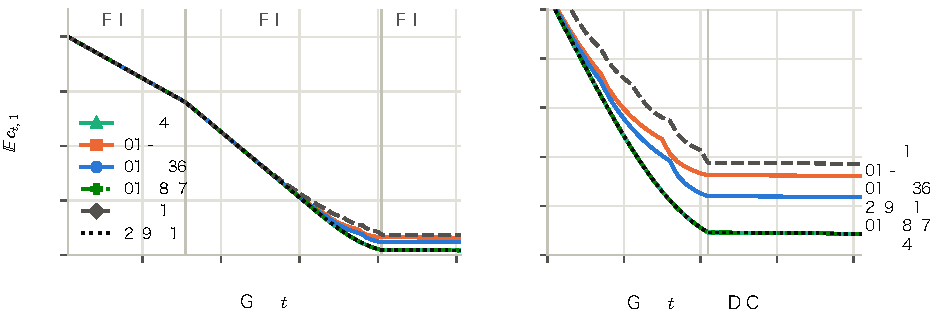
\includegraphics[width=\linewidth]{figures/order_b213.pdf}
\caption{顺序 $2\to1\to3$ 下商品 1 的期望库存 $\E c_{t,1}$。竖线为类型分块的边界，右图为第 60 期之后的局部放大}
\label{fig:order}
\end{figure}

\subsection{库存水平与推荐位数}\label{sec:sens}
把三种商品的库存同比例缩放为 $\lfloor\theta C\rceil$（四舍五入），在五份数据上精确评价各策略，结果见表\ref{tab:theta}与图\ref{fig:theta}。

\begin{table}[htbp]
\centering\footnotesize
\caption{库存缩放 $C\to\lfloor\theta C\rceil$ 下的策略损失（五份数据平均）}\label{tab:theta}
\begin{tabular}{ccrrrrrrrr}
\toprule
$\theta$ & $C$ & $F$ & $\overline{V^{\seq}}$ & $\overline L^{\AlgOne}$ & $\overline L^{\Greedy}$ & $\overline L^{\LPFD}$ & $\overline L^{\LPDual}$ & $\overline L^{\IIDDP}$ & $\overline W^{\AlgOne}$ \\
\midrule
0.3 & $(12,\,11,\,8)$ & 256.0 & 255.996 & 0.173 & 0.006 & 0.006 & 0.006 & 0.000 & 125.81 \\
0.4 & $(16,\,14,\,10)$ & 332.0 & 331.954 & 1.236 & 0.111 & 0.111 & 0.111 & 0.000 & 104.58 \\
0.5 & $(20,\,18,\,13)$ & 422.0 & 421.226 & 7.945 & 1.796 & 1.583 & 1.583 & 0.003 & 80.29 \\
0.6 & $(24,\,21,\,15)$ & 498.0 & 494.473 & 15.256 & 5.685 & 3.174 & 3.174 & 0.067 & 62.04 \\
0.7 & $(28,\,25,\,18)$ & 578.0 & 567.598 & 18.769 & 8.638 & 3.888 & 3.609 & 0.335 & 41.79 \\
0.8 & $(32,\,28,\,20)$ & 629.0 & 618.196 & 12.434 & 4.723 & 1.643 & 1.665 & 0.328 & 26.80 \\
0.9 & $(36,\,32,\,23)$ & 670.0 & 663.494 & 6.250 & 1.521 & 0.738 & 0.457 & 0.289 & 13.99 \\
1.0 & $(40,\,35,\,25)$ & 706.0 & 696.062 & 2.669 & 0.513 & 0.572 & 0.169 & 0.201 & 6.29 \\
1.1 & $(44,\,39,\,28)$ & 724.0 & 715.337 & 0.684 & 0.099 & 0.265 & 0.042 & 0.076 & 1.90 \\
1.2 & $(48,\,42,\,30)$ & 724.0 & 722.424 & 0.107 & 0.012 & 0.064 & 0.006 & 0.016 & 0.35 \\
\bottomrule
\end{tabular}
\end{table}


\begin{figure}[htbp]
\centering
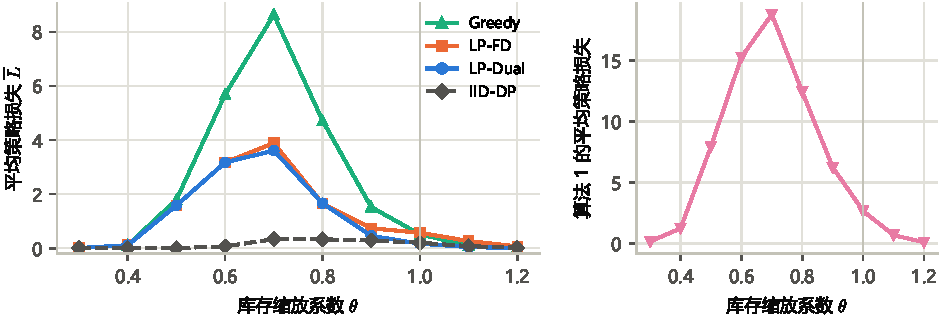
\includegraphics[width=\linewidth]{figures/theta.pdf}
\caption{库存缩放下的平均策略损失（左）与算法 1 的平均策略损失（右）}
\label{fig:theta}
\end{figure}

库存水平决定了在线决策的难度。$\theta\le0.4$ 时三种商品都严重短缺，每件库存几乎都能售出，除算法 1 外各策略都接近最优；$\theta\ge1.1$ 时库存几乎不构成约束，\Greedy{} 已接近最优。中间区域的库存分配最关键：$\theta=0.7$ 时 \Greedy{} 的策略损失达到 \ThetaSevenLGreedy，\LPDual{} 降至 \ThetaSevenLDual，\IIDDP{} 只有 \ThetaSevenLIID。两种 LP 策略在 $\theta\le0.9$ 时表现接近，课程实例 $\theta=1$ 附近的差别来自第\ref{sec:where}节分析的期末过度预留。$\theta=0.6$--$0.8$ 时，LP 策略与 \IIDDP{} 之间仍有约 1.3--3.3 的差距。损失分解显示，$\theta=0.7$ 时 \LPDual{} 的 \LossThetaSevenDual{} 策略损失中有 \SellThetaSevenDual{} 是类型 1 多卖。此时开始的对偶价格为 $\beta=(9,5,0)$，类型 1 顾客对三种商品的评分都是 $0.6$，三者并列，按即时收益推荐了商品 1、2。动态规划的判断不同：库存紧张时商品 1 迟早会售罄，暂不卖给当前的类型 1 顾客几乎没有损失（后来的类型 1 顾客仍会买走它），却保留了卖给类型 2 顾客的机会。流体模型只比较期望值，看不到这种由需求波动产生的期权价值，随机动态规划在库存紧张时因此仍有改进空间。

算法 1 的损失随库存减少而迅速上升。$\theta=0.5$ 时，它平均每条路径推荐 \ThetaHalfW{} 次缺货商品（共 200 个推荐位），策略损失为 \ThetaHalfLAlg；损失在 $\theta=0.7$ 时达到 \ThetaSevenLAlg。这从数量上回答了问题一：库存越紧张，忽略库存造成的损失越大。

\begin{proposition}\label{prop:kn}
当 $K\ge n$ 时，每期推荐全部有货且 $p_{ij}>0$ 的商品在每条样本路径上都达到最大收入
\begin{equation}
R^{*}=\sum_{j=1}^{n}r_j\min\Bigl\{C_j,\ \sum_{t=1}^{T}\ind\{J_t=j\}\Bigr\}.
\end{equation}
\end{proposition}
\begin{proof}
任何策略售出的商品 $j$ 都不超过初始库存，也不超过首选为 $j$ 的顾客人数。推荐全部有货商品时，商品 $j$ 售罄之前每位首选 $j$ 的顾客都会购买，因此销量恰好等于两者中的较小值。
\end{proof}

\begin{table}[htbp]
\centering\small
\caption{推荐位数 $K$ 对期望收入的影响（五份数据平均）}\label{tab:K}
\begin{tabular}{crrrrrrr}
\toprule
$K$ & $F$ & $\overline{V^{\seq}}$ & $\overline{\E R}^{\AlgOne}$ & $\overline{\E R}^{\Greedy}$ & $\overline{\E R}^{\LPFD}$ & $\overline{\E R}^{\LPDual}$ & $\overline{\E R}^{\IIDDP}$ \\
\midrule
1 & 492.0 & 491.992 & 462.772 & 478.001 & 487.070 & 484.848 & 491.992 \\
2 & 706.0 & 696.062 & 693.394 & 695.550 & 695.490 & 695.894 & 695.862 \\
3 & 734.0 & 727.810 & 727.810 & 727.810 & 727.810 & 727.810 & 727.810 \\
\bottomrule
\end{tabular}
\end{table}


表\ref{tab:K}比较了不同推荐位数。$K=3=n$ 时，五种在线策略都推荐全部有货商品（算法 1 推荐全部商品，缺货商品不影响其余商品的成交），期望收入都等于 \KERthreeDual{}，与命题\ref{prop:kn}一致。$K=1$ 时策略之间差异最大：\Greedy{} 为 \KERoneGreedy，\LPDual{} 为 \KERoneDual，\LPFD{} 为 \KERoneFD，\IIDDP{} 达到 \SeqDP{} 的 \KVone。损失几乎全部来自同一类决策：类型 2 顾客对商品 1、2 的即时收益相同（$v_{21}=v_{22}=4$），只有一个推荐位时应当推荐库存充裕的商品 2，把商品 1 留给偏好它的类型 1 顾客。$K=1$ 时类型 1 顾客只看到商品 1，对它的流体需求为 $0.3\tau$。只要 $c_1\ge0.3\tau$，流体模型就认为商品 1 不稀缺，对偶价格为零，类型 2 顾客的两件商品评分并列（均为 4.0），按编号推荐商品 1；$c_1$ 降到 $0.3\tau$ 以下后对偶价格变为正数，才转向商品 2。结果是 \LPDual{} 把商品 1 的库存维持在类型 1 期望需求附近，类型 1 的随机需求超过它时，部分类型 1 顾客买不到商品 1。实际上，向类型 2 推荐商品 2 没有任何代价，\IIDDP{} 从不向类型 2 推荐商品 1。\LPFD{} 的有限差分在库存接近流体需求时先变为正数，较早转向商品 2，损失较小（\LossKoneFD{}，\LPDual{} 为 \LossKoneDual）。这一现象说明，流体模型不重视安全库存：期望需求略低于库存时，它把多余的库存视为零价值。评分并列时以剩余库存作为次级排序依据，是一个可能的改进方向。

\subsection{规模扩展与计算时间}\label{sec:scale}
\textbf{课程实例上的计算时间。} 主实验共 100 万次决策，借助按 $(\tau,c^{\tau})$ 的缓存，\LPDual{} 共求解 \SolvesDual{} 个线性规划，\LPFD{} 求解 \SolvesFD{} 个。不命中缓存的决策中，\LPDual{} 的决策时间中位数为 \TimeDualMedian{} 毫秒，95\% 分位数为 \TimeDualP{} 毫秒；\LPFD{} 分别为 \TimeFDMedian{} 毫秒和 \TimeFDP{} 毫秒。

\textbf{销售期放大。} 把销售期放大为 $T$，库存同比例放大为 $\lfloor TC/100\rceil$，每个 $T$ 生成 10 条人数为 $T\lambda$ 的随机排列并模拟，结果见表\ref{tab:scaling}。\LPDual{} 的遗憾估计在 $T$ 从 25 增至 \ScaleTmax{} 的过程中处于 \ScaleGDualMin--\ScaleGDualMax{} 之间，没有随 $T$ 增长的趋势。$T$ 较大时单条路径收入的标准差随 $\sqrt T$ 增大，遗憾估计的置信半宽随之变宽（$T=\ScaleTmax$ 时为 \ScaleDualHwMax），但 $\overline R^{\LPDual}/F$ 从 $T=25$ 的 95\% 升至 $T=\ScaleTmax$ 的 \ScaleRatioMax\%，相对遗憾持续下降，符合流体近似在大规模下趋于准确的一般结论\cite{gallego,jasin}。\Greedy{} 则不同。在流体近似下，\Greedy{} 以 $0.5\times0.6+0.3\times0.4=0.42$ 的速率消耗商品 1，在 $t^{*}=0.4T/0.42$ 时售罄，此前每期期望收入为 7.24；此后类型 1 改看 $\{2,3\}$，类型 2 只剩商品 2 可买，每期期望收入降为 3.34。商品 2、3 的消耗分别不超过 $0.29T$ 与 $0.13T$，在销售期内不会售罄。于是
\begin{equation}
F-R^{\Greedy}_{\mathrm{fluid}}=7.06\,T-\bigl[7.24\,t^{*}+3.34\,(T-t^{*})\bigr]\approx0.0057\,T,
\label{eq:greedyfluid}
\end{equation}
即 \Greedy{} 的遗憾中有一项随 $T$ 线性增长。单个策略的遗憾估计噪声太大，看不出这一趋势；公共随机数下的配对差则精确得多。表\ref{tab:scaling}中，$T\le100$ 时 \LPDual{} 与 \Greedy{} 的配对收益差不超过 \ScaleGapSmall，此后随 $T$ 近似线性扩大，$T=\ScaleTmax$ 时为 $\ScaleGreedyGapMax\pm\ScaleGreedyGapMaxHw$，与式\eqref{eq:greedyfluid}给出的 \ScaleGreedyFluid{} 量级一致。课程实例的 $T=100$ 规模较小，这一差异被需求波动掩盖；销售期越长、顾客越多，考虑库存机会成本的收益越明显。

\begin{table}[htbp]
\centering\footnotesize
\caption{销售期与库存同比例放大时的遗憾}\label{tab:scaling}
\begin{tabular}{rcrrrrrrr}
\toprule
$T$ & $C$ & $F$ & $\widehat G^{\Greedy}$ & $\widehat G^{\LPFD}$ & $\widehat G^{\LPDual}\pm h$ & $\bar d^{\,\LPDual,\Greedy}\pm h$ & $\overline{F-V^{\seq}}$ & $\overline R^{\LPDual}/F$ \\
\midrule
25 & $(10,9,6)$ & 178 & 8.80 & 9.01 & $8.63\pm0.62$ & $0.17\pm0.09$ & 8.19 & 95.14\% \\
50 & $(20,18,13)$ & 353 & 8.46 & 8.74 & $8.32\pm0.87$ & $0.14\pm0.12$ & 8.60 & 97.64\% \\
100 & $(40,35,25)$ & 706 & 11.30 & 11.34 & $10.94\pm1.02$ & $0.36\pm0.11$ & 9.77 & 98.45\% \\
200 & $(80,70,50)$ & 1412 & 10.22 & 9.73 & $9.66\pm1.81$ & $0.56\pm0.18$ & 9.72 & 99.32\% \\
400 & $(160,140,100)$ & 2824 & 8.86 & 7.56 & $7.50\pm2.67$ & $1.36\pm0.32$ & -- & 99.73\% \\
800 & $(320,280,200)$ & 5648 & 10.26 & 7.29 & $7.57\pm4.61$ & $2.69\pm0.45$ & -- & 99.87\% \\
1600 & $(640,560,400)$ & 11296 & 10.01 & 2.88 & $3.45\pm4.85$ & $6.55\pm0.91$ & -- & 99.97\% \\
\bottomrule
\end{tabular}
\par\vspace{0.35em}{\footnotesize 各 $T$ 独立生成 10 条固定人数的随机排列，人数按 $T\lambda$ 取整后使总和等于 $T$。每条序列模拟 300 次购买（$T=800$ 时 150 次，$T=1600$ 时 100 次），策略共享购买抽样。$\widehat G=F-\overline R$。以每条序列的模拟均值或配对差均值为一个观测，$h$ 是 10 条独立序列间的 95\% $t$ 区间半宽。$T>200$ 时未计算 $V^{\seq}$。}
\end{table}


\textbf{较大的随机实例。} 按 Dirichlet 分布生成购买概率（含不购买选项），价格为 4--20 的整数，到达率也按 Dirichlet 分布生成，库存取算法 1 期望需求的 $\rho$ 倍，$\rho\in\{0.6,0.9\}$，结果见表\ref{tab:large}。这组实验主要检验可行性与计算时间：
\begin{itemize}
\item \textbf{可行性。} 在全部 \LargeInstances{} 个实例、5 种维度组合上，三种库存感知策略都没有推荐缺货商品；算法 1 每条路径平均出现数十到数百次缺货推荐，收入只有离线上界的 \LargeAlgOneMin\%--\LargeAlgOneMax\%，而 \Greedy{} 不低于 \LargeGreedyMin\%。这再次说明问题一中库存过滤的必要性。
\item \textbf{计算时间。} 最大配置的线性规划有 \LargeVars{} 个变量、\LargeRows{} 条约束，处于受限许可证的规模之内。\LPDual{} 的单期决策时间中位数为 \LargeTimeMedian{} 毫秒，95\% 分位数为 \LargeTimeP{} 毫秒；\LPFD{} 每期需要求解至多 $n+1=31$ 个线性规划，中位数为 \LargeTimeFD{} 毫秒。
\item \textbf{收入。} 各配置下 \LPDual{} 相对 \Greedy{} 的平均配对收入差在离线上界的 \LargePairMin\% 与 \LargePairMax\% 之间；逐个实例检验，\LPDual{} 显著较高的有 \LargeSigWins{} 个，显著较低的有 \LargeSigLosses{} 个。这些实例的状态空间过大，无法计算 $V^{\seq}$ 来分解遗憾；从配对差看，库存机会成本带来的改进与课程实例一样较小，且在不同实例上方向不一，不能据此断言 \LPDual{} 在一般实例上优于 \Greedy{}。第\ref{sec:sens}节的灵敏度分析表明，改进的大小取决于库存的紧张程度和顾客偏好的冲突程度。
\end{itemize}

\begin{table}[htbp]
\centering\footnotesize
\caption{随机生成的较大实例}\label{tab:large}
\begin{tabular}{lrrrrrrrrrr}
\toprule
 & & \multicolumn{4}{c}{$\overline R/F$ (\%)} & (\%) & & \multicolumn{3}{c}{单期决策时间/ms} \\
\cmidrule(lr){3-6}\cmidrule(lr){9-11}
$(m,n,T,K)$ & $\rho$ & \AlgOne & \Greedy & \LPFD & \LPDual & $\bar d/F\pm h$ & $\overline W^{\AlgOne}$ & $t^{\LPDual}_{50}$ & $t^{\LPDual}_{95}$ & $t^{\LPFD}_{50}$ \\
\midrule
$(2,5,50,1)$ & 0.6 & 81.9 & 95.6 & 95.4 & 95.9 & $0.29\pm0.17$ & 21 & 0.01 & 0.61 & 0.01 \\
$(2,5,50,1)$ & 0.9 & 90.6 & 96.3 & 96.5 & 96.5 & $0.18\pm0.21$ & 9 & 0.01 & 0.72 & 0.01 \\
$(3,6,100,2)$ & 0.6 & 94.6 & 98.3 & 98.5 & 98.5 & $0.20\pm0.11$ & 81 & 0.52 & 1.14 & 1.04 \\
$(3,6,100,2)$ & 0.9 & 94.0 & 96.7 & 96.6 & 96.7 & $0.00\pm0.14$ & 32 & 0.56 & 1.17 & 1.77 \\
$(5,10,100,3)$ & 0.6 & 92.4 & 97.8 & 97.7 & 97.7 & $-0.07\pm0.06$ & 125 & 0.68 & 1.38 & 2.25 \\
$(5,10,100,3)$ & 0.9 & 89.0 & 92.4 & 92.0 & 92.3 & $0.00\pm0.19$ & 56 & 0.81 & 1.78 & 3.52 \\
$(10,20,200,5)$ & 0.6 & 94.1 & 98.5 & 98.5 & 98.5 & $0.00\pm0.02$ & 424 & 1.33 & 2.66 & 7.02 \\
$(10,20,200,5)$ & 0.9 & 88.4 & 92.4 & 92.1 & 92.4 & $0.00\pm0.15$ & 208 & 1.77 & 3.90 & 11.81 \\
$(20,30,300,4)$ & 0.6 & 90.7 & 98.4 & 98.4 & 98.4 & $-0.02\pm0.06$ & 513 & 2.93 & 5.27 & 22.26 \\
$(20,30,300,4)$ & 0.9 & 84.5 & 91.1 & 91.3 & 91.4 & $0.32\pm0.27$ & 258 & 3.61 & 4.86 & 28.96 \\
\bottomrule
\end{tabular}
\par\vspace{0.35em}{\footnotesize 每种配置随机生成 8 个实例，每个实例 60 次购买重复（$m=20$ 时减半），各策略使用公共随机数。$\rho$ 为库存相对于算法 1 期望需求的比例；$\bar d/F$ 为 \LPDual{} 减 \Greedy{} 的配对收入差占 $F$ 的百分比，$h$ 为 95\% 置信半宽；$\overline W$ 为每条路径上缺货推荐的平均次数；$t_{50}$、$t_{95}$ 为单期决策时间的中位数与 95\% 分位数，包含线性规划求解与排序。}
\end{table}


\section{结论}\label{sec:conclusion}
本文对题目的三个问题给出如下回答。

\textbf{问题一。} 有限库存下不能直接使用算法 1。它不检查库存，售罄商品会持续占用推荐位，既违反零缺货推荐的要求，也浪费了展示其他商品的机会。算例\ref{ex:q1}中，算法 1 相对一个简单可行策略的收入损失在 $T\ge14$ 时超过 30\%，$T=20$ 时为 47.08\%，并随 $T$ 增大趋于 100\%。课程实例上，库存同比例缩小到一半时，算法 1 平均每条路径推荐 \ThetaHalfW{} 次缺货商品。

\textbf{问题二。} 含库存约束的离线模型是流体线性规划\eqref{eq:lp}，它在题目模型中加入期望库存约束，并把推荐决策放松为比例。该模型给出任意在线策略期望收入的上界，课程实例的最优值为 706，影子价格 $\beta^{*}=(9,0,0)$ 表明商品 1 是唯一的稀缺资源，其机会成本来自类型 1 顾客改看商品 3 的代价。

\textbf{问题三。} \LPDual{} 每期重新求解一次剩余销售期的流体线性规划，以库存对偶价格作为机会成本，在有货商品中按调整后收益推荐。策略在每条路径上满足库存约束，每期至多求解一个含 $mn$ 个变量的连续线性规划。五份数据上，\LPDual{} 的平均和最大期望遗憾为 \GavgDual{} 和 \GmaxDual，均低于库存感知贪心（\GavgGreedy、\GmaxGreedy）与有限差分策略（\GavgFD、\GmaxFD）。相对贪心的平均收入提高了 \DualGreedyAvg{}，与预知到达序列最优策略的差距缩小了 \DualSeqGapReductionPct\%。

数值实验还给出以下几点认识。
\begin{enumerate}[label=(\arabic*)]
\item \textbf{购买波动限制了可达收入。} 五份数据上，流体上界 706 与预知顾客顺序时的最优期望收入 \ERSeq{} 之间相差 \FluidGap。商品 1 的随机需求是一个具体来源。这个差额占 \LPDual{} 平均期望遗憾的 \FluidShare\%；从该策略到预知序列最优决策的差额为 \LavgDual。
\item \textbf{同比例放大课程实例时，机会成本的作用更明显。} 在按比例放大的流体模型中，贪心路径与流体最优解的收入差为约 $0.0057T$。在随机购买模拟中，$T=\ScaleTmax$ 时 \LPDual{} 相对贪心的平均配对增收为 $\ScaleGreedyGapMax\pm\ScaleGreedyGapMaxHw$（95\% 置信区间半宽）。最大规模随机配置中，先对每个实例求单期决策时间的第 95 百分位数，再对实例取平均，结果为 \LargeTimeP{} 毫秒（原实验环境）。
\item \textbf{库存条件会改变展示失误的代价。} 在五份课程数据中，逐期损失分解表明，\Greedy{} 的主要失误是向类型 1 过早出售商品 1，\LPFD{} 的主要失误是期末预留过多。沿库存缩放网格观察，算法 1 的缺货展示随库存收紧而增多，其收入损失在中度紧张时达到峰值。
\item \textbf{集中到达会使固定到达率预测失准。} 到达顺序为 $2\to1\to3$ 时，依赖到达率的策略为不会再出现的类型 2 顾客预留库存，期望收入降至 \BlockDual；改用剩余人数预测后恢复到 \BlockCount。
\item \textbf{流体近似看不到需求波动带来的价值。} 流体模型按期望需求预留库存，而课程实例中多留一件的代价约为少留一件的 9 倍，最优预留量远低于期望需求，因此在 $1\to2\to3$ 顺序下，准确的人数预测反而使 \LPCount{} 多留、收入降至 \BlockOTTCount。另一方面，对偶价格使混合使用的推荐集合恰好无差异，库存紧张时（$\theta=0.7$）按即时收益打破并列会多卖；只有一个推荐位时，流体模型又把安全库存视为零价值。这些情形下，LP 策略与随机动态规划之间有 1--7 的差距。
\end{enumerate}

本文的局限与可能的改进方向：购买模型假定顾客不在推荐集合内替代；需求预测只使用固定到达率或总人数；对偶价格在退化点不唯一，评分并列时的规则会影响结果。后续可以考虑在线估计到达率，在并列时按剩余库存排序，或在状态空间较小时用近似动态规划修正流体模型的机会成本。


\begin{thebibliography}{99}
\bibitem{assignment} Online Top-K Recommendation. 课程项目题目, 2026.
\bibitem{gallego} Gallego G, van Ryzin G. A multiproduct dynamic pricing problem and its applications to network yield management. \textit{Operations Research}, 1997, 45(1): 24--41.
\bibitem{talluri98} Talluri K, van Ryzin G. An analysis of bid-price controls for network revenue management. \textit{Management Science}, 1998, 44(11): 1577--1593.
\bibitem{talluribook} Talluri K, van Ryzin G. \textit{The Theory and Practice of Revenue Management}. New York: Springer, 2004.
\bibitem{jasin} Jasin S, Kumar S. A re-solving heuristic with bounded revenue loss for network revenue management with customer choice. \textit{Mathematics of Operations Research}, 2012, 37(2): 313--345.
\bibitem{golrezaei} Golrezaei N, Nazerzadeh H, Rusmevichientong P. Real-time optimization of personalized assortments. \textit{Management Science}, 2014, 60(6): 1532--1551.
\bibitem{bumpensanti} Bumpensanti P, Wang H. A re-solving heuristic with uniformly bounded loss for network revenue management. \textit{Management Science}, 2020, 66(7): 2993--3009.
\bibitem{gurobi} Gurobi Optimization. \textit{Gurobi Optimizer Reference Manual}, Version 13.0. 2026.
\end{thebibliography}

\appendix
\section{程序结构与运行}\label{app:code}
全部代码位于 \texttt{code} 目录。原实验使用 Python 3.11，修订时在 Python 3.12 和 Gurobi 13.0.3 环境复核；依赖见 \texttt{requirements.txt}。在线算法求解连续线性规划，最大规模的扩展实验含 600 个变量。第\ref{sec:q2}节另以两个离线整数模型作对照。
\begin{itemize}
\item \texttt{recommendation.py}：实例定义 \texttt{Instance}、可复用的流体线性规划 \texttt{FluidLP}、四种在线策略（\texttt{FixedTopK} 即算法 1、\texttt{Greedy}、\texttt{LPLookahead}、\texttt{LPDual}）、公共随机数模拟器 \texttt{simulate}、动态规划 \texttt{dp\_benchmark}，以及精确评价所需的 \texttt{exact\_forward} 与 \texttt{LPTables}。
\item \texttt{run\_policy.py}：对任意到达序列 CSV（列 \texttt{t}, \texttt{i\_t}）运行指定策略，输出逐期推荐、购买、库存轨迹，以及总收入、剩余库存、hindsight 与遗憾；可通过 JSON 文件指定任意 $m,n,T,K$ 的实例。
\item \texttt{experiments.py}：第\ref{sec:q1}节、第\ref{sec:q2}节与第\ref{sec:exp}节的全部实验，随机种子固定。
\item \texttt{make\_assets.py}：读取 \texttt{results} 目录中的结果，生成论文的表格、图形与数值宏。
\item \texttt{tests.py}：自动化测试。
\end{itemize}
常用命令如下（在 \texttt{code} 目录下运行）：
\begin{verbatim}
python run_policy.py "../online recommendation/data/arrivals_dataset_1.csv"
python run_policy.py my_arrivals.csv --reps 1000
python run_policy.py my_arrivals.csv --policy LP-FD --instance instance.json
python tests.py
python experiments.py all
python make_assets.py
\end{verbatim}
在线服务中，平台创建一次策略对象，每期调用 \texttt{recommend(i, c, H)} 得到推荐集合，其中 \texttt{i} 为顾客类型（从 0 开始编号），\texttt{c} 为当前库存，\texttt{H} 为含本期在内的剩余期数；观察到购买结果后由平台更新库存。

\section{自动化测试}\label{app:tests}
在 conda base 的 Python 3.12.7 与 Gurobi 13.0.3 环境中执行 \texttt{python tests.py}，17 项测试全部通过。下表列出各组的验收内容。
\begin{center}
\small
\begin{tabularx}{\linewidth}{@{}l r X@{}}
\toprule
测试组 & 项数 & 核对内容 \\
\midrule
流体模型 & 4 & 课程实例的目标值 706、销量和原始对偶相等；商品与推荐集合两种 LP 等价；五段库存价格及四个断点；两期反例的固定方案、在线最优和流体值分别为 0.6、0.84、1。\\
动态规划 & 2 & 递归枚举与 Bellman 方程相符，前向传播与后向递推对贪心、独立到达策略和预知序列策略给出相同收入。\\
策略与模拟 & 10 & 在线推荐与动作表、向量化与逐项排序、剩余人数预测与购买模拟相互核对。涵盖单期只累计一次到达、不同维度的可行性和前缀因果性、缺货展示、购买概率、零分并列、全商品展示与非法输入。\\
反例 & 1 & 题一中固定推荐和可行策略的闭式期望收入与精确计算一致。\\
\bottomrule
\end{tabularx}
\end{center}

剩余人数预测的回归例含 18 期、三类顾客人数 $(8,5,5)$。逐状态枚举在每期只登记一次当期顾客，期末计数恢复为 $(8,5,5)$，对偶策略的期望收入为 110.618000，与独立构造的动作表一致。

\end{document}
